
\documentclass[lang=cn,newtx,10pt,scheme=chinese]{elegantbook}
\title{AIGC}
\subtitle{扩散模型}

\author{Sisyphes}
\institute{家里蹲}
\date{\today}
\version{0.1}

\setcounter{tocdepth}{3}

\logo{logo-blue.png}
\cover{cover.jpg}

% 本文档命令
\usepackage{array}
\newcommand{\ccr}[1]{\makecell{{\color{#1}\rule{1cm}{1cm}}}}

% 修改标题页的橙色带
\definecolor{customcolor}{RGB}{32,178,170}
\colorlet{coverlinecolor}{customcolor}
\usepackage{cprotect}

\addbibresource[location=local]{reference.bib} % 参考文献,不要删除

\begin{document}

\maketitle
\frontmatter

\tableofcontents

\mainmatter

\chapter{零}
\section{符号说明}
\begin{itemize}
    \item 采样步数 $s$
    \item 噪声 $z$
    \item 参数 $\theta$
    \item 原始样本 $x_0$
    \item  扰动核: $p_\sigma(\tilde{\mathbf{x}} \mid \mathbf{x}):=\mathcal{N}\left(\tilde{\mathbf{x}} ;\mathbf{x}, \sigma^2 \mathbf{I}\right)$
    \item 扰动数据分布:$p_\sigma(\tilde{\mathbf{x}}):=\int p_{\text {data }}(\mathbf{x})p_\sigma(\tilde{\mathbf{x}} \mid \mathbf{x}) \mathbf{d} \mathbf{x}$
    \item 扰动数据的分布分数:$\nabla_{\mathbf{x}} \log p_{\alpha_i}(\mathbf{x})$
    \item 噪声条件网络优化目标:$\boldsymbol{\theta}^*=\underset{\boldsymbol{\theta}}{\arg \min } \sum_{i=1}^N \sigma_i^2 \mathbb{E}_{p_{\mathbf{data}}(\mathbf{x})} \mathbb{E}_{p_{\sigma_i}(\tilde{\mathbf{x}} \mid \mathbf{x})}\left[\left\|\mathbf{s}_{\boldsymbol{\theta}}\left(\tilde{\mathbf{x}}, \sigma_i\right)-\nabla_{\tilde{\mathbf{x}}} \log p_{\sigma_i}(\tilde{\mathbf{x}} \mid \mathbf{x})\right\|_2^2\right]$
    \item  原始数据分布: $p_x$, 先验分布 $p_T$
    \item 连续采样步数:$t \in [0, T]$
    \item 连续扩散过程的变量:${x(t)}_{t=0}^{T}$
    \item 离散扩散过程变量:
    \item Itô SDE:$\mathbf{d} \mathbf{x}=\mathbf{f}(\mathbf{x}, t) \mathbf{d} t+g(t) \mathbf{d} \mathbf{w}$
    \item  前向SDE:$\mathbf{d} \mathbf{x}=\mathbf{f}(\mathbf{x}, t) \mathbf{d} t+g(t) \mathbf{d} \mathbf{w}$
    \item $x(t)$的drift coefficient:$\mathbf{f}(\cdot, t): \mathbb{R}^d \rightarrow \mathbb{R}^d$
    \item $x(t)$的diffusion coefficient:$g(\cdot):\mathbb{R} \rightarrow \mathbb{R}$
    \item 反向SDE:$\mathbf{d} x=\left[f(x, t)-g^2(t) \nabla_x \log p_t(x)\right] \mathbf{d} t+g(t) \mathbf{d} \bar{w}$,其中$\bar{w}$是标准维纳过程,时间从$T$到$0$,$dt$也是负向。
    \item standard Wiener proces(Brownian motion):$\boldsymbol{w}$
    \item $\mathbf{x}(s)$到$\mathbf{x}(t)$的转移核:$p_{s t}(\mathbf{x}(t) \mid \mathbf{x}(s)),0 \leqslant s<t \leqslant T$
    \item probability flow ODE
    \item ELBO 

\end{itemize}
\section{一些废话}
不重复生产,因此部分使用了两个博客的原文部分内容,和一些研究者的见解,在统一符号上做了一些调整。
\subsection{无中生有}
。
\subsection{翻译}
将问题翻译为计算机数学语言,将计算机数学语言翻译为数学语言,将代数翻译为几何,将模糊翻译为半模糊,
将清晰翻译为模糊,将模糊翻译为模糊,将模糊翻译为清晰,将公式翻译为比喻,将公式翻译为代码,
将代码翻译为业务代码,将论文翻译为项目,将项目翻译为产品部分...

\chapter{总体介绍}

\begin{itemize}
  \item 模板官网:\href{https://elegantlatex.org/}{elegantlatex.org}
  \item 模板GitHub 地址:\href{https://github.com/ElegantLaTeX/}{ElegantLaTeX}
  \item 项目地址:\href{https://github.com/foocker}{Sisyphes}
  \item 作图工具:\href{https://www.geogebra.org/?lang=en}{geogebra}
\end{itemize}

\section{基本介绍}



\section{学术进展}
\begin{enumerate}
  \item \href{https://lilianweng.github.io/posts/2021-07-11-diffusion-models/}{什么是扩散模型}
  \item \href{http://yang-song.net/blog/2021/score/}{什么是分数生成模型}
  \item \href{https://arxiv.org/abs/1907.05600}{NCSN Yang, Ermon, 2019}
  \item \href{https://arxiv.org/abs/2006.11239}{DDPM; Ho et al. 2020}
  \item \href{https://www.stats.ox.ac.uk/~teh/research/compstats/WelTeh2011a.pdf}{stochastic gradient Langevin dynamics Welling , Teh 2011}
  \item \href{http://www.iro.umontreal.ca/~vincentp/Publications/smdae_techreport.pdf}{denoising/slice score matching 2011}
  \item \href{https://arxiv.org/abs/1503.03585}{Deep Unsupervised Learning using Nonequilibrium Thermodynamics 2015}
  \item \href{https://arxiv.org/abs/2102.09672}{Improved Denoising Diffusion Probabilistic Models 2021}
  \item \href{https://arxiv.org/abs/2112.10752}{High-Resolution Image Synthesis with Latent Diffusion Models 2022}
  \item \href{https://openreview.net/forum?id=qw8AKxfYbI}{Classifier-Free Diffusion Guidance 2021}
  \item \href{https://sassafras13.github.io/ReparamTrick/}{Reparameterization Trick}
  \item \href{https://kexue.fm/archives/6705}{漫谈重参数:从正态分布到Gumbel Softmax}
  \item \href{https://github.com/YangLing0818/Diffusion-Models-Papers-Survey-Taxonomy}{SD综述和应用}
  \item \href{https://github.com/facebookincubator/AITemplate/tree/main/examples/05_stable_diffusion}{AIT-SD}
  \item \href{https://github.com/NVIDIA/TensorRT/tree/release/8.6/demo/Diffusion}{TRT-SD}
  \item \href{https://github.com/Oneflow-Inc/diffusers}{Oneflow-SD}
  \item \href{https://github.com/huggingface/peft}{PEFT}
\end{enumerate}

\chapter{数学基础}

\section{高斯分布、熵,KL散度、重参数}

\href{https://en.wikipedia.org/wiki/Evidence_lower_bound}{Evidence lower bound}
定义:设$X, Z$ 是随机变量,其联合分布为$p_{\theta}$.比如$p_{\theta}(X)$是关于$X$的边缘分布,$p_{\theta}(Z|X)$是给定$X$关于$Z$的条件分布。于是有,对于样本$x \sim p_{\theta}$,对任意分布$q_{\phi}$,其ELBO定义为:
\begin{equation}
L(\phi, \theta ; x):=\mathbb{E}_{z \sim q_\phi(\cdot \mid x)}\left[\ln \frac{p_\theta(x, z)}{q_\phi(z \mid x)}\right]
\end{equation}
等价形式为:

\begin{equation}
\begin{aligned}
L(\phi, \theta ; x) & 
=\mathbb{E}_{z \sim q_\phi(\cdot \mid x)}\left[\ln p_\theta(x, z)
\right]+H\left[q_\phi(z \mid x)\right] \\ & 
=\ln p_\theta(x)-D_{K L}\left(q_\phi(z \mid x) \| p_\theta(z \mid x)\right) .
\end{aligned}
\end{equation}

其中$H$表示熵,$\ln p_{\theta}$为$x$的证据,而KL散度恒大于0,因此
$\ln p_{\theta} \geq \mathbb{E}_{z \sim q_\phi(\cdot \mid x)}
\left[\ln \frac{p_\theta(x, z)}{q_\phi(z \mid x)}\right]
$

\href{https://github.com/janishar/mit-deep-learning-book-pdf}{deeplearningbook 2016} 或者
\href{https://www.deeplearningbook.org/contents/autoencoders.html}{deeplearningbook 2016 autoencoders} 
从中了解到,VLB和ELBO在定义上存在一个正负符号只差。
\href{https://github.com/goodfeli/dlbook_notation}{dlbook notation 2016}

\href{https://www.inf.ed.ac.uk/teaching/courses/fmcs1/slides/lecture25.pdf}
\href{https://en.wikipedia.org/wiki/Entropy\_(information\_theory)}{Entropy information theory }

\begin{equation}
\mathbf{H}(X):=-\sum_{x \in \mathcal{X}} p(x) \log p(x)
\end{equation}

\href{https://planetmath.org/shannonsentropy}{shannonsentropy}。

两个一元高斯分布的KL散度公式:
\begin{equation}
K L\left(\mathcal{N}\left(\mu_1, \sigma_1^2\right)|| 
\mathcal{N}\left(\mu_2, \sigma_2^2\right)\right)=
\log \frac{\sigma_2}{\sigma_1}-\frac{1}{2}+\frac{\sigma_1^2+
\left(\mu_1-\mu_2\right)^2}{2 \sigma_2^2}
\end{equation}

多元的参考:\href{https://mr-easy.github.io/2020-04-16-kl-divergence-between-2-gaussian-distributions/}{kl-divergence-between-2-gaussian-distributions}

重参数技巧:\href{https://lilianweng.github.io/posts/2018-08-12-vae/#reparameterization-trick}{reparameterization-trick}

\section{贝叶斯定理}
关于先验,后验,极大似然,似然函数等

\section{Fisher score 、Stein score}
Fisher score
\href{https://zh.wikipedia.org/wiki/%E8%B4%B9%E5%B8%8C%E5%B0%94%E4%BF%A1%E6%81%AF}{费希尔信息}

Stein score 
\href{https://projecteuclid.org/ebooks/berkeley-symposium-on-mathematical-statistics-and-probability/Proceedings-of-the-Sixth-Berkeley-Symposium-on-Mathematical-Statistics-and/chapter/A-bound-for-the-error-in-the-normal-approximation-to/bsmsp/1200514239}{A bound for the error in the normal approximation to
the distribution of a sum of dependent random variables. 1972}
\href{http://proceedings.mlr.press/v48/chwialkowski16.pdf}{A Kernel Test of Goodness of Fit 2016}
\href{https://arxiv.org/pdf/1602.03253.pdf}{A Kernelized Stein Discrepancy for Goodness-of-fit Tests 2016}
定义2.1给出了概率分布$p$的Stein score function。该定义从Stein 1972年写的一篇文章中抽取出来,相关内容可参考\href{https://en.wikipedia.org/wiki/Stein%27s_method}{Stein's method}。


\section{Markov chain Monte Carlo}
\href{https://zhuanlan.zhihu.com/p/37121528}{马尔可夫链蒙特卡罗算法(MCMC)}
\href{https://web.math.ucsb.edu/~atzberg/pmwiki_intranet/uploads/AtzbergerHomePage/Atzberger_MonteCarlo.pdf}{The Monte-Carlo Method}
\href{https://en.wikipedia.org/wiki/Markov_chain_Monte_Carlo}{Markov chain Monte Carlo}

\section{证据下界或变分下界}
对于给定前向过程,
$q\left(\mathbf{x}_t \mid \mathbf{x}_{t-1}\right)=\mathcal{N}\left(\mathbf{x}_t ; \sqrt{1-\beta_t} \mathbf{x}_{t-1}, 
\beta_t \mathbf{I}\right) \quad q\left(\mathbf{x}_{1: T} \mid \mathbf{x}_0\right)=
\prod_{t=1}^T q\left(\mathbf{x}_t \mid \mathbf{x}_{t-1}\right)$,
逆向过程用$p_{\theta}$表示,
$p_\theta\left(\mathbf{x}_{0: T}\right)=p\left(\mathbf{x}_T\right) 
\prod_{t=1}^T p_\theta\left(\mathbf{x}_{t-1} \mid \mathbf{x}_t\right) \quad p_\theta\left(\mathbf{x}_{t-1} \mid \mathbf{x}_t\right)=
\mathcal{N}\left(\mathbf{x}_{t-1} ; 
\boldsymbol{\mu}_\theta\left(\mathbf{x}_t, t\right), \mathbf{\Sigma}_\theta\left(\mathbf{x}_t, t\right)\right)
$,
数据的负对数似然为$-log_{p_{\theta}}(x_0)$,$x_0$属于训练数据空间中的元素,一种常见的变分下界推导方式是给负对数似然增加一个恒大于0的变量,
关于在给定数据的情况下,过程数据的条件联合分布函数 从正向和反向两个角度得到,他们的KL散度值。加上这个项,整个就能训练了,因此可叫训练项目。
\begin{equation}
  \begin{aligned}
    -\log p_\theta\left(\mathbf{x}_0\right) 
    & \leq-\log p_\theta\left(\mathbf{x}_0\right)+D_{\mathbf{KL}}\left(q\left(\mathbf{x}_{1: T} \mid \mathbf{x}_0\right) \| p_\theta\left(\mathbf{x}_{1: T} \mid \mathbf{x}_0\right)\right) \\ 
    & =-\log p_\theta\left(\mathbf{x}_0\right)+\mathbb{E}_{\mathbf{x}_{1: T} \sim q\left(\mathbf{x}_{1: T} \mid \mathbf{x}_0\right)}\left[\log \frac{q\left(\mathbf{x}_{1: T} 
    \mid \mathbf{x}_0\right)}{p_\theta\left(\mathbf{x}_{0: T}\right) / p_\theta\left(\mathbf{x}_0\right)}\right] \\ 
    & =-\log p_\theta\left(\mathbf{x}_0\right)+\mathbb{E}_q\left[\log \frac{q\left(\mathbf{x}_{1: T} \mid \mathbf{x}_0\right)}{p_\theta\left(\mathbf{x}_{0: T}\right)}+\log p_\theta\left(\mathbf{x}_0\right)\right] \\ 
    & =\mathbb{E}_q\left[\log \frac{q\left(\mathbf{x}_{1: T} \mid \mathbf{x}_0\right)}{p_\theta\left(\mathbf{x}_{0: T}\right)}\right] \\ \text { Let } L_{\mathbf{VLB}} & =\mathbb{E}_{q\left(\mathbf{x}_{0: T}\right)}
    \left[\log \frac{q\left(\mathbf{x}_{1: T} \mid \mathbf{x}_0\right)}{p_\theta\left(\mathbf{x}_{0: T}\right)}\right] 
    \geq-\mathbb{E}_{q\left(\mathbf{x}_0\right)} \log p_\theta\left(\mathbf{x}_0\right)
  \end{aligned}
\end{equation}

从交叉熵的角度,根据Jensen's不等式,也能得出变分下界:
\begin{equation}
  \begin{aligned} L_{\mathbf{CE}} 
    & =-\mathbb{E}_{q\left(\mathbf{x}_0\right)} \log p_\theta\left(\mathbf{x}_0\right) \\ 
    & =-\mathbb{E}_{q\left(\mathbf{x}_0\right)} \log \left(\int p_\theta\left(\mathbf{x}_{0: T}\right) d \mathbf{x}_{1: T}\right) \\ 
    & =-\mathbb{E}_{q\left(\mathbf{x}_0\right)} \log \left(\int q\left(\mathbf{x}_{1: T} \mid \mathbf{x}_0\right) \frac{p_\theta\left(\mathbf{x}_{0: T}\right)}{q\left(\mathbf{x}_{1: T} \mid \mathbf{x}_0\right)} d \mathbf{x}_{1: T}\right) \\ 
    & =-\mathbb{E}_{q\left(\mathbf{x}_0\right)} \log \left(\mathbb{E}_{q\left(\mathbf{x}_{1: T} \mid \mathbf{x}_0\right)} \frac{p_\theta\left(\mathbf{x}_{0: T}\right)}{q\left(\mathbf{x}_{1: T} \mid \mathbf{x}_0\right)}\right) \\ 
    & \leq-\mathbb{E}_{q\left(\mathbf{x}_{0: T}\right)} \log \frac{p_\theta\left(\mathbf{x}_{0: T}\right)}{q\left(\mathbf{x}_{1: T} \mid \mathbf{x}_0\right)} \\ 
    & =\mathbb{E}_{q\left(\mathbf{x}_{0: T}\right)}\left[\log \frac{q\left(\mathbf{x}_{1: T} \mid \mathbf{x}_0\right)}{p_\theta\left(\mathbf{x}_{0: T}\right)}\right]=L_{\mathbf{VLB}}
  \end{aligned}
\end{equation}
通过一步一步的推导,多步变分下界 可以写为 多个KL散度和熵的和。这一过程,原因在于扩散扩散的一条马尔科夫链。
整个过程是比较简单的,核心在等式第五行的一个贝叶斯转换,转换的原因在于给定扩散过程,逆向转移在给定$x_0$的基础上,能被具体的计算出来。

\begin{equation}
  \begin{aligned} & 
    \text { Attention }(\mathbf{Q}, \mathbf{K}, \mathbf{V})=\operatorname{softmax}\left(\frac{\mathbf{Q K}^{\top}}{\sqrt{d}}\right) \cdot \mathbf{V} \\ 
    & \text { where } \mathbf{Q}=\mathbf{W}_Q^{(i)} \cdot \varphi_i\left(\mathbf{z}_i\right), \mathbf{K}=\mathbf{W}_K^{(i)} \cdot \tau_\theta(y), \mathbf{V}=\mathbf{W}_V^{(i)} \cdot \tau_\theta(y) \\ 
    & \text { and } \mathbf{W}_Q^{(i)} \in \mathbb{R}^{d \times d_e^i}, \mathbf{W}_K^{(i)}, \mathbf{W}_V^{(i)} \in \mathbb{R}^{d \times d_r}, \varphi_i\left(\mathbf{z}_i\right) \in \mathbb{R}^{N \times d_c^i}, \tau_\theta(y) \in \mathbb{R}^{M \times d_r}
  \end{aligned}
\end{equation}

\begin{equation}
  \begin{aligned} \mathbf{KL}\left(p_0(\mathbf{x}) \| p_\theta(\mathbf{x})\right) \leq \frac{T}{2} \mathbb{E}_{t \in \mathcal{U}(0, T)} \mathbb{E}_{p_t(\mathbf{x})}\left[\lambda(t) \| \nabla_{\mathbf{x}} \log p_t(\mathbf{x})-\right. 
    & \left.\mathbf{s}_\theta(\mathbf{x}, t) \|_2^2\right] \\ + 
    & \operatorname{KL}\left(p_T \| \pi\right)
  \end{aligned}
\end{equation}

\section{SDE 和ODE}
简单介绍下。

概率流常微分的迹,
随机微分方程的边缘概率密度,以及这两者的关系。
从同样的数据分布采样,迹有同样的边缘分布?
概率流常微分的半边结构。

% \newpage
% \begin{problemset}
%   \item 完成一个RL与动作控制的开源项目
% \end{problemset}


\chapter{扩散模型}

\section{整体认识}
\begin{itemize}
  % \item \href{}{}
  \item  Fisher divergence $\mathbb{E}_{p(\mathbf{x})}\left[\left\|\nabla_{\mathbf{x}} \log p(\mathbf{x})-\mathbf{s}_\theta(\mathbf{x})\right\|_2^2\right]=\int p(\mathbf{x})\left\|\nabla_{\mathbf{x}} \log p(\mathbf{x})-\mathbf{s}_\theta(\mathbf{x})\right\|_2^2 \mathbf{~d} \mathbf{x}$
  \item score matching
  \item  Langevin dynamics
  \item \href{c}{Correlation functions and computer simulations 1981}
  \item \href{c}{Correlation functions and computer simulations 1994}
  \item \href{c}{A Kernel Test of Goodness of Fit 2016}
  \item \href{c}{A kernelized Stein discrepancy for goodness-of-fit tests 2016}
  \item $\mathbf{x}_{i+1} \leftarrow \mathbf{x}_i+\epsilon \nabla_{\mathbf{x}} \log p(\mathbf{x})+\sqrt{2 \epsilon} \mathbf{z}_i, \quad i=0,1, \cdots, K$, 从任意分布$\mathbf{x}_0 \sim \pi(\mathbf{x})$出发,其中$z_i$服从标准正太分布,
  $\epsilon \rightarrow 0, K \rightarrow \infty$,分数模型的MCMC采样(郎之万动力),收敛到$p(\mathbf{x})$。分数模型$\mathbf{s}_\theta(\mathbf{x}) \approx \nabla_{\mathbf{x}} \log p(\mathbf{x})$是通过score-matching(分数匹配算法)得到,
  不需要难处理的常数化因子,核心是优化Fisher divergence,score-matching规避了对 Stein score function的具体计算。
  通过score matching去训练一个 score-based model,然后使用Langevin dynamics采样得到服从目标分布的数据。但是这种理论上的逻辑,
  在实际操作中,会有分数模型在低密度区精度很差(从积分公式上看到,率密度权重因子),另外分数模型是对高维张量的求导,因此在实际处理中需要做计算量的简化。
  解决方案是用噪声扰动数据点,并在噪声数据点上训练基于分数的模型。当噪声强度足够大的时候,噪声可以填充低数据密度区域,以提高估计分数的准确性。
  论文参考。
  $p_{\sigma_i}(\mathbf{x})=\int p(\mathbf{y}) \mathcal{N}\left(\mathbf{x} ; \mathbf{y}, \sigma_i^2 I\right) \mathbf{d} \mathbf{y}$,
  从$p(\mathbf{x})$中采样,然后使用重参数得到$p_{\sigma_i}(\mathbf{x})$中的样本,其中$\sigma_i$是噪声方差,且递增。
  \item \href{c}{Generative Modeling by Estimating Gradients of the Data Distribution 2019}
  \item \href{c.c}{Sliced score matching: A scalable approach to density and score estimation 2020}
  \item \href{c}{Improved Techniques for Training Score-Based Generative Models 2020}
  \item \href{c}{Score-Based Generative Modeling through Stochastic Differential Equations 2021} 训练目标变
  为:$\mathbf{s}_\theta(\mathbf{x}, i) \approx \nabla_{\mathbf{x}} \log p_{\sigma_i}(\mathbf{x})$ 
  for all $i=1,2, \cdots, L$, $\sum_{i=1}^L \lambda(i) \mathbb{E}_{p_{\sigma_i}(\mathbf{x})}
  \left[\left\|\nabla_{\mathbf{x}} \log p_{\sigma_i}(\mathbf{x})-\mathbf{s}_\theta(\mathbf{x}, i)
  \right\|_2^2\right]$,噪声$\mathcal{N}\left(0, \sigma_i^2 I\right), i=1,2, \cdots, L
  $上面式子使用score-matching来训练。log-likelihood(对数似然)的计算,
  这里先验是$p_T(\mathbf{x})$,利用n.c, s.c中的定理1和等式4,可以利用ODE的数值求解,在先验概率密度$p_T$已知的情况下,
  计算未知数据$\mathbf{x}$的概率密度$p_0$,得到数据的对数似然。这里和贝叶斯中的似然函数,有区别。在上面的设定中,
  似然函数是$p(\mathbf{x}|\mathbf{\epsilon})$,其中$\mathbf{\epsilon}$是标准正太分布的噪声,
  而对数似然是根据数据得到的带参数$\theta$的关于数据的概率密度函数,在某些情况下,你可以把这里的$\mathbf{\epsilon}$看
  做参数$\theta$,但这里还是有区别的。
  \item \href{c.c}{Maximum Likelihood Training of Score-Based Diffusion Models 2021}
  
  \item \href{B.D}{Reverse-time diffusion equation models 1982}
  \item \href{c.c}{A connection between score matching and denoising autoencoders 2011} 
  \item \href{n.c}{Neural Ordinary Differential Equations 2018}
  \item \href{s.c}{Scalable Reversible Generative Models with Free-form Continuous Dynamics 2019}
  \item variational dequantization to obtain likelihoods on discrete images
  \item 求关于不好计算的东西的的其他变量的导数,将不好计算的量消去,变为从导数的角度来刻画该问题。
  \item 生成模型的逆向问题,或者贝叶斯推理问题:设随机变量$\mathbf{x}, \mathbf{y}$,设计
  好前向$\mathbf{x} \rightarrow \mathbf{y}$,于是其转移概率$p(\mathbf{y}|\mathbf{x})$已知,逆向
  问题是计算$p(\mathbf{x}|\mathbf{y})$。根据贝叶斯法则:$p(\mathbf{x} \mid \mathbf{y})=p(\mathbf{x}) p(\mathbf{y} 
  \mid \mathbf{x}) / \int p(\mathbf{x}) p(\mathbf{y} \mid \mathbf{x}) \mathbf{d} \mathbf{x}$。设$\mathbf{x}$为先验,
  则后验若按照贝叶斯法则,但积分项难于计算,若两边对$\mathbf{x}$求导,即$\nabla_{\mathbf{x}} \log p(\mathbf{x} \mid \mathbf{y})=\nabla_{\mathbf{x}} \log p(\mathbf{x})+\nabla_{\mathbf{x}} \log p(\mathbf{y} \mid \mathbf{x})$,容易看到利用score matching 和Langevin-type采样能直接得到后验分数函数值。
  \item 公式翻译,理论和应用间的近似和区别,模糊地方的经验法则,代码上的并行考虑,部署上的性能考虑,应用上的扩展性,资源的考虑。
  \item 分数模型是从分数匹配和郎之万动力采样中得到的,而扩散模型是有证据下界ELBO和解码模型采样得到的。
  而ELBO训练的扩散模型和分数模型是等价的。这个是在2020年提出DDPM之后,2021年宋飏等证明的,并提出了SDE的统一架构。
  这种不同角度对同一任务的描述,类似量子力学中的波函数角度和矩阵力学角度最终被证明是等价的类似,来个更简单点的,
  单位圆盘上的有理数点的无穷性和本原勾股数的无穷性是等价的。
  \item 基于分数模型的成功关键:
  (1)使用多个噪声尺度的扰动数据,并为每个噪声尺度训练基于分数的模型;
  (2)使用U-Net架构(我们使用RefineNet,因为它是现代版本的基于分数的模型;
  (3)将朗之万MCMC应用于每个噪声尺度,并将它们链接在一起。
  \item 基于分数的生成模型,只能用在连续数据上,若离散数据,可先利用VAE将其映射到连续的隐空间中,
  然后训练分数模型,最后解码。对于分数模型采样速度慢的问题,可以利用ODE的快速求解,来克服。 
  \item 基于分数的生成模型或扩散模型:数据生成,密度估计,逆问题求解。
  \item ELBO或VLB(两者是同种东西的不同说法),分别叫证据下界,变分下界。变分下界来自VAE模型的说法,
  而且扩散模型本身,也可以看成多步VAE模型。但实际上,这里面存在一些正负符号的区别,有误用嫌疑。
  
  \item \href{https://arxiv.org/abs/2112.10752}{LDM 2022} 
  
  \item \href{https://arxiv.org/pdf/2206.00364.pdf}{Elucidating the Design Space of Diffusion-Based Generative Models }
  对当前的几种diffusion model做了一个统一的框架。解决了diffusion ODE的生成效果一直都不如diffusion SDE,效果反而更好。
  但,实际上是个大杂烩(这点我和Baof观点相同)。
  \item \href{https://arxiv.org/abs/2201.06503}{Analytic-DPM}
  “DDPM的均值实际上是对diffusion SDE的maximum likelihood SDE solver,并且最优方差有解析形式,且可以被score function唯一确定。
  最优方差也可以用score model来近似。”
  \item \href{https://github.com/LuChengTHU/dpm-solver}{dpm-solver}, 
  \href{https://arxiv.org/pdf/2211.01095.pdf}{DPM-SOLVER++}
  “证明了DDIM是diffusion ODE的一阶ODE solver,并且提出了二阶、三阶solver,可以做到10步采样质量很不错,20步几乎收敛。
  不需要任何额外训练,任给一个pretrained model都可以直接用。 DDIM对应了diffusion ODE的1阶ODE solver,它的加速效果
  好是因为它考虑了ODE的半线性结构,而DPM-Solver给出了对应的更高阶的solver,可以让10步左右的采样达到与DDPM的1000步的采样相当。”
  \item \href{https://arxiv.org/pdf/2206.08265.pdf}{Maximum Likelihood Training for Score-Based Diffusion ODEs by High-Order Denoising Score Matching} 
  “从理论角度彻底分析出了Diffusion SDE与Diffusion ODE的最大似然训练的联系和区别,并且提出了新的二阶、三阶denoising score matching算法来
  解决了diffusion ODE的最大似然训练问题。结论就是,之前训练diffusion model的“去噪”方法其实是一阶score matching,它只适合训
  练diffusion SDE的最大似然估计,但并不适合训练diffusion ODE的最大似然估计。想要对diffusion ODE做最大似然估计,需要采用上面提出的方法。”
  \item “深度生成模型除了可以生成数据以外,还有一类核心任务是估计数据的概率密度(可以用模型计算的数据似然(likelihood)来刻画)。GAN被诟病的一点就是无法计算似然,因为它是隐式生成模型(implicit generative model),这导致GAN无法被用来数据压缩等领域。而VAE只能计算数据似然的一个下界,也不太令人满意。”
  \item “DDPM与上文提到的连续版本的reverse SDE可以称为diffusion SDE(也叫Score-based SDE),它们都是基于SDE(离散版本为条件高斯分布)定义的生成模型。然而,这类模型与VAE一样,无法计算精确的数据似然(likelihood),而只能计算ELBO。Diffusion model的另一个优势是,只要训练了score model(上文提到的三种等价形式都可以转换为score model),那么就可以导出一个Neural ODE,它是一类continuous normalizing flow,可以精确计算数据的似然。”

  \item "然后说说我认为diffusion model的美妙之处。它把困难的数据生成,拆分成了若干个相对简单的任务,每个任务即对应一次去噪。这种拆分有坏处(即推断慢,但我们的工作一定程度上解决了这个问题),也有好处(更加可控的生成)。"

  \item 一个东西,有一些框架,发展到一定时候,会出现新的框架。
  \item \href{https://ml.cs.tsinghua.edu.cn/~fanbao/Application-DPM.pdf}{PPT}
  \item 问题,NCSN是如何训练的? 和DDPM训练有啥区别?
  \item DDIM是使用的NCSN或变分去噪的训练方式,但论文公式推导是使用的$V\_LB$思路
  \item Analysis-DPM是在DDIM的基础上分析了其其实可以计算出中间的最优均值和方差
  \item DPM-solver是将SDE对应推出来的ODE的常微分方程,做了具体的计算,加速了推理采样速度,
  但是中间公式的推导却使用的是DDPM原始的表示,而非分数模型,虽然做了两者的等价变换。
  \item DPM-solver++是在DPM-solver的基础上,对guide 做了分析,但是在公式推导过程中,
  做了DDPM模型的$x_0$替换,使得最终表示出来的微分方程,在高阶部分的展开不同。不过这个替
  换的核心原因,似乎是来自Photorealistic text-to-image diffusion models with deep 
  language understanding 2022b这篇文章的启发,该文章实验出,对输入变量的尺度变换,能有效
  抑制数据的边界范围溢出的情况,而且采样生成的数据效果确实更好了。从直观上,论文也做了两点分析,主要是$s$因子,
  带来的尺度上的变化。
  \item 我比较好奇的是,使用的是DDPM的建模思路,但具体公式推导上采用的是SDE的模型表示,或者反之,做一些替换,前
  者建模是从贝叶斯,极大似然,的思路,做变分界的推导,后者是从分数模型对应的SDE的逆向推导,虽然两者得到的模型在效
  果上等价的,刻画了原始数据的分布,但是,彼此互换,就能解决不同的问题,有点迷。
  \item 分数模型SGM的训练是预测噪声除以方差,同DDPM差不多,不过SGM设置添加的噪声服从高斯分布,但没假设其满足马尔
  科夫性。通过sliced score matching 训练NCSN,即去噪分数匹配。推理使用nnealed Langevin dynamics。
  \item 分数模型的建模思路和DDPM的建模思路不同,前者通过分数匹配优化,郎之万动力采样,后者通过贝叶斯,极大似然的变
  分下界 优化,"逆向"采样。 但二者的连续版本 被SDE 统一。而SDE有对应的ODE,其解能保持SDE的所有边缘分布,从而对OD
  E的求解,能极大提高推理的速度。
  \item 在连续化DDPM和SGM的时候,就去掉了DDPM的马尔科夫性的假设,虽然DDIM也是去掉了DDPM的前向的马尔科夫性假设,但
  同时假设了与 DDPM设定前向为马尔科夫性之后,推导出的逆向中条件后验分布为高斯分布 同等形式的 高斯分布。DDIM是通过
  什么,带来的推理加速(逆向采样几乎一样,多了一个$\sigma^2_{t}$,在附录C.1中说明了是通过DDPM的逆采样的子序列采样
  得到)? 但是奇怪的是,DDIM的训练,竟然是变分去噪或者分数模型。其实差不多,这点需要代码上确认下区别。在实际中,DDIM
  的效果并不怎么样,后续的SDE均比它好很多。
  \item It is well-known that maximizing the log-likelihood of a probabilistic model is equivalent to m
  inimizing the KL divergence from the data distribution to the model distribution.
  \item 在特殊的权重因子上,极小化SDE的分布与数据分布的KL散度的上界,其上界是和分数匹配相关的损失,从而达到优化
  分数模型来提高数据的似然函数值的精度。并且,优化组合分数匹配损失,并不能直接得到数据的对数似然函数,通过概率流模
  型continuous normalizing flows (CNFs)优化SGM能得到SGM的极大似然值,并且提高其似然函数值的准确性。ScoreFlow。
  \item SDE的模型是不能计算似然值的,但是ODE是可以精确就算的。优化一阶分数损失并不能得到ODE的似然,负对数似然被
  ODE的一阶,二阶,三阶分数误差所控制。因此一种高阶的去噪分数匹配算法能达到更精确的似然估计。具体来说和SDE类似的计
  算了模型和数据的散度,并在ODE这块,得到了类似的优化界。SDE被$J_{SM}$控制,ODE被$J_{SM}, J_{Fisher}$两者控制。
  这里有个具体的方格例子,可以测试下。ScoreODEs。 问题,似然函数的具体计算,意味着啥?这里也是隐含计算的,并且只
  针对连续值,实际的值需要做量化处理,量化处理靠谱吗?经过仔细分析了吗?可以分析还是类似于以前分类网络的感知损失这
  种参考评估?
  \item sliced  score matching:分数模型的估计在参数估计不一致,估计方差较大,实现繁琐,三方面的改进。提出了投影
  分数函数到随机向量然后做比较的方法。从而能处理更高维的数据,更复杂的分布。核心思路是拟合高维函数在不同方向上的投影。
  文章也做了理论分析,在一些正则条件下,能做到一致的和渐近正态的参数估计,是一个良定义的统计估计标准。(能量)密度估计
  和分数估计。整个文章可以理解为:对2005年文章Hyvärinen (2005))中,梯度迹的估计。但是仍然要前向$n$次。理论上是这样,
  但是实际上sliced  score matching的损失还是非常不稳定的,若增加了噪声,就稳定多了。
  \item 极大似然对unnormalized  models的优化,存在难以处理的归一化分母$Z_\theta$,对其做关于$x$的微分,则消除了该
  问题,于是问题转化为拟合被称为分数函数的问题,但同时也带来了计算复杂的问题,黑塞矩阵(Hessian),论文思路启发自
  Sliced Wasserstein distance (Rabin et al., 2012),
  \item Denoising Score Matching(2011)彻底克服了需要计算Hessian的问题。但是论文只是考虑了一次加噪声,后续论文NCSN
  是做了多次加噪。相关对分数匹配在高维上的优化,还有Approximate Backpropagation,Curvature  Propagation等不同
  类型文章。Denoising Score Matching是估计扰动后的数据的分数。sliced score matching是对未扰动的数据的分数估计,
  但是计算量大了几倍。
  \item NCSN, 郎之万动力采样:从分数模型中采样得到符合原始数据分布的数据。数据本身是嵌入在高维流形中的低维流形,
  而分数函数是在原始空间高维流形中计算梯度的,当数据被限制在低维流形中时,该微分是无定义的,其次分数匹配的优化目标
  能优化出一个一致性分数估计的前提是,数据分布的支撑集得是整个空间,当数据集中在低维流形时,该估计是不一致的。低密
  度区域的数据,不仅导致分数的估计偏差,而且使得郎之万动力采样结果不准确。因此添加噪声,不仅能保证数据集的支撑是整个
  空间,而且更大的噪声,能减少低密度区域的出现。使得分数估计定义良好,且估计准确,采样准确。通过添加多尺度的噪声,
  使得噪声扰动分布逼近到真实数据分布。这将通过,训练一个拟合所有尺度噪声的模型。采样从大尺度噪声逐渐过渡到小尺度噪声。
  添加也是从大噪声到小噪声,直到数据变为高斯分布。

\end{itemize}

\subsection{问题}
\begin{itemize}
    \item 马尔科夫过程对任意分布都能变换的定理
    \item 分数模型的训练
    \item SMLD,DDPM的 SDE化细节
    \item  Langevin MCMC
    \item 前向SDE的逆向由什么定理得到
    \item 条件逆过程
    \item progressive distillation
    \item classifier-free guidance(CFG)
\end{itemize}


\section{离散版DDPM等}
\begin{figure}[h!]
\centering
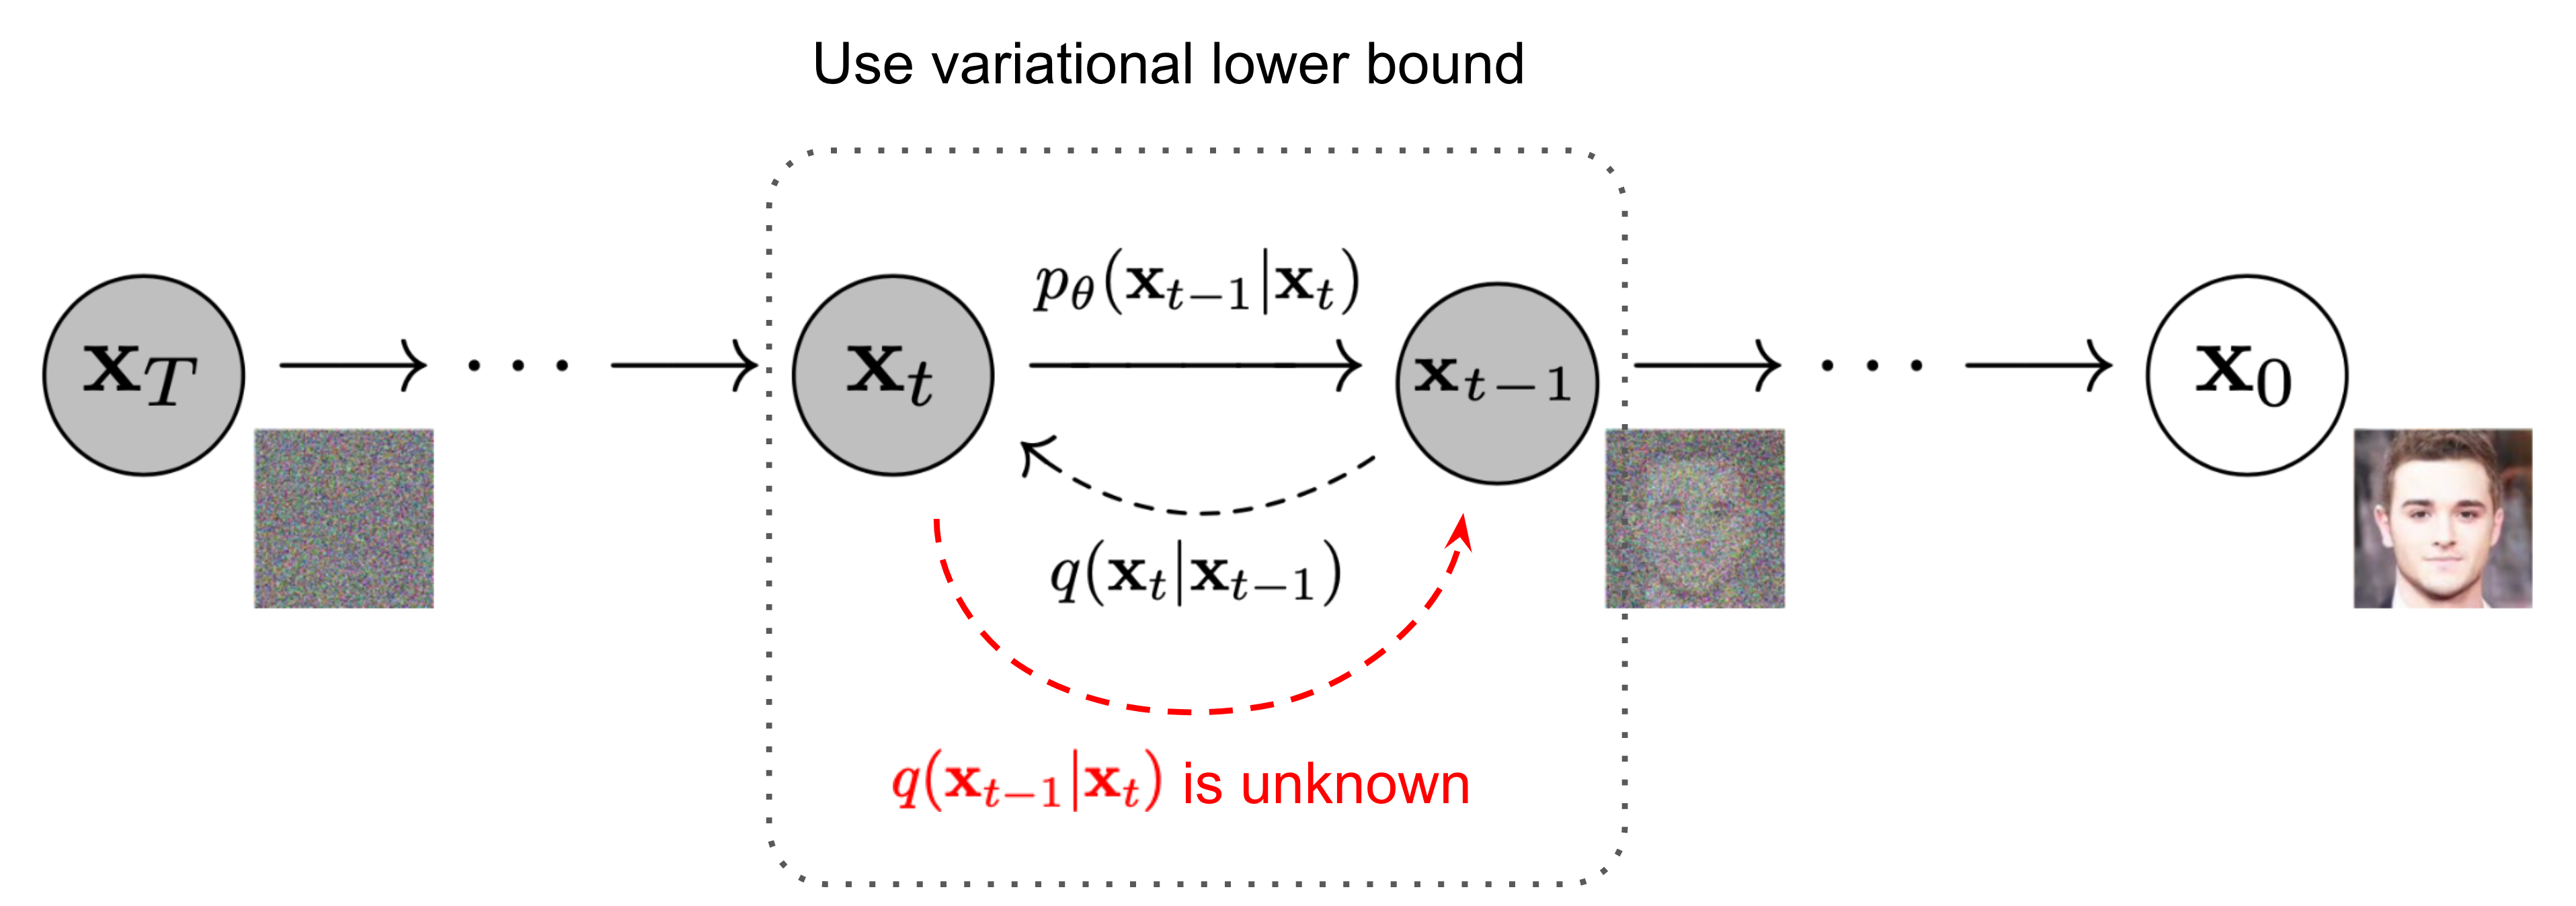
\includegraphics[scale=0.15]{image/DDPM.png}
\caption{DDPM}
\label{fig:DDPM}
\end{figure}

真实数据分布$\mathbf{x}_0 \sim q (\mathbf{x})$,这里的$x_0$可能是$512*512*3$大小的图像集合,也可能是$\mathbb{R}^{n}$中的向量,比如动画BVH解析出的数据表示。

前向扩散过程定义为$T$步的马尔科夫过程,转移概率为$q(\mathbf{x}_t|\mathbf{x}_{t-1}), t \in \mathbb{N}$。对于给定数据$\mathbf{x}_0$,向其添加同维度的高斯样本(微小扰动),然后递推。设置好每一步添加样本的均值和方差,使得输入样本$x_0$变为标准正太分布的样本,如图4.1所示。比如序列$\left\{\beta_t \in(0,1)\right\}_{t=1}^T, \beta_1 < \beta_2 < \cdots < \beta_T\}$,将转移概率(条件概率)定义为$q\left(\mathbf{x}_t \mid \mathbf{x}_{t-1}\right)=\mathcal{N}\left(\mathbf{x}_t ; \sqrt{1-\beta_t} \mathbf{x}_{t-1}, \beta_t \mathbf{I}\right)$ 容易看到,当$T \rightarrow \infty$时,$q(\mathbf{x}_t|\mathbf{x}_{t-1})$趋近于标准状态分布。

令
\begin{equation}
\alpha_t = 1 - \beta_t, \bar{\alpha_{t}} = \prod_{i=1}^{t}\alpha_i,
\end{equation}
对于$q\left(\mathbf{x}_t \mid \mathbf{x}_{t-1}\right)$,由重参数化得
$\mathbf{x}_t =\sqrt{\alpha_t} \mathbf{x}_{t-1}+\sqrt{1-\alpha_t} \epsilon_{t-1}$,
又由高斯分布的叠加特性,可得
$\mathbf{x_0} \rightarrow \mathbf{x_t}$的转化:
\begin{equation}
\begin{array}{rlr}
\mathbf{x}_t & =\sqrt{\alpha_t} \mathbf{x}_{t-1}+\sqrt{1-\alpha_t} \epsilon_{t-1} & \quad ;  \epsilon_{t-1}, \epsilon_{t-2}, \cdots \sim \mathcal{N}(\mathbf{0}, \mathbf{I}) \\
& =\sqrt{\alpha_t \alpha_{t-1}} \mathbf{x}_{t-2}+\sqrt{1-\alpha_t \alpha_{t-1}} \bar{\epsilon}_{t-2}  \\
& =\cdots & \\
& =\sqrt{\bar{\alpha}_t} \mathbf{x}_0+\sqrt{1-\bar{\alpha}_t} \boldsymbol{\epsilon}
\end{array}
\end{equation}
其中合并的高斯分布$\bar{\epsilon}_{t-2} = \sqrt{\alpha_{t}(1-\alpha_{t-1})}\epsilon_{t-2} + \sqrt{1-\alpha_t}\epsilon_{t-1}$。
于是得到
\begin{equation}
q\left(\mathbf{x}_t \mid \mathbf{x}_0\right)=\mathcal{N}\left(\mathbf{x}_t ; \sqrt{\bar{\alpha}_t} \mathbf{x}_0,\left(1-\bar{\alpha}_t\right) \mathbf{I}\right)
\end{equation}
根据变换关系,有$\bar{\alpha_1} > \cdots > \bar{\alpha_T}$。

前向过程:人为设计一个马尔科夫扩散过程,将任意分布(有限维度),在有限步数之内,逼近一个标准正太分布。

关于DL的建模,可以简单理解为将目标转化特定的语言体系,然后在该体系中构建一个闭环,而且需要梳理一下闭环中的链接关系,并在优化中把这些关系体现出来。

这里的任务是生成训练数据对应空间的样本,由贝叶斯定理,
只要知道$q(\mathbf{x}_t \mid \mathbf{x}_{t-1}), t=1,\cdots, T$整个链条闭环就有了。首先数据的分布$q(\mathbf{x}_0)$是未知的,
且数据分布是我们的目标,但我们会准备很多数据,所以可以假想$q(\mathbf{x}_0)$已知,又前向是已知的,于是,整个链条中,
只剩下反向$q(\mathbf{x}_t \mid \mathbf{x}_{t-1})$,可用参数模型$\mathcal{N}\left(\mathbf{x}_{t-1} ;
 \boldsymbol{\mu}_\theta\left(\mathbf{x}_t, t\right), \boldsymbol{\Sigma}_\theta\left(\mathbf{x}_t, t\right)\right)$来表示。

前向和反向的闭环,前向:
\begin{equation}
q\left(\mathbf{x}_0, \mathbf{x}_1, \cdots, \mathbf{x}_T\right)=q(\mathbf{x}_{0:T}):=q\left(\mathbf{x}_0\right) \prod_{t=1}^T q\left(\mathbf{x}_t \mid \mathbf{x}_{t-1}\right)
\end{equation}
反向:
\begin{equation}
p_\theta\left(\mathbf{x}_0, \mathbf{x}_1, \cdots, \mathbf{x}_T\right)=p_\theta(\mathbf{x}_{0:T}):=p\left(\mathbf{x}_T\right) \prod_{t=1}^T p_\theta\left(\mathbf{x}_{t-1} \mid \mathbf{x}_t\right)
\end{equation}
这两者相等,因为它们都是表示初始数据和中间数据的联合分布。
要优化这两分布,就要找一个刻画两分布的距离的函数。其中KL散度,交叉熵,Stein's score函数均可。
对于KL散度,有
\begin{equation}
\begin{aligned}
& \quad \mathbf{KL}\left(q\left(\mathbf{x}_0, \mathbf{x}_1, \cdots, \mathbf{x}_T\right) \| p_\theta\left(\mathbf{x}_0, \mathbf{x}_1, \cdots, \mathbf{x}_T\right)\right) \\
& \stackrel{(i)}{=}-\mathbb{E}_{q\left(\mathbf{x}_0, \mathbf{x}_1, \cdots, \mathbf{x}_T\right)}\left[\log p_\theta\left(\mathbf{x}_0, \mathbf{x}_1, \cdots, \mathbf{x}_T\right)\right]+\mathbf{const} \\
& \stackrel{(i i)}{=} \underbrace{\mathbb{E}_{q\left(\mathbf{x}_0, \mathbf{x}_1, \cdots, \mathbf{x}_T\right)}\left[-\log p\left(\mathbf{x}_T\right)-\sum_{t=1}^T \log \frac{p_\theta\left(\mathbf{x}_{t-1} \mid \mathbf{x}_t\right)}{q\left(\mathbf{x}_t \mid \mathbf{x}_{t-1}\right)}\right]}_{:=-L_{\mathbf{VLB}}\left(\mathbf{x}_0\right)}+\mathbf{const} \\
& \stackrel{(i i i)}{\geq} \mathbb{E}\left[-\log p_\theta\left(\mathbf{x}_0\right)\right]+\text { const, }
\end{aligned}
\end{equation}

这里需要说明一下,很多地方说变分下界VLB和证据下界是一样的,包括Wikipedia,但实际上Wikipedia关于ELBO的定义和一些扩散论文对VLB的定义
能看出来,两者差一个正负符号(这里面应该存在一些误用)。

从式(4.6)的推导中看到
\begin{equation}
\log \frac{p_\theta\left(\mathbf{x}_{t-1} \mid \mathbf{x}_t\right)}{q\left(\mathbf{x}_t \mid \mathbf{x}_{t-1}\right)}
\end{equation}
是关键。这里前向$q(\mathbf{x}_t \mid \mathbf{x}_{t-1})$均值、方差已知,而逆向我们假设也满足高斯分布,
利用网络$\mathbf{s}_\theta(\mathbf{x}_t, t)$来表示它。当前情况可以做优化,但是实际没有选择这个,而是考虑到前向的马尔可夫性,
有$q(\mathbf{x}_t \mid \mathbf{x}_{t-1})=q(\mathbf{x}_t \mid \mathbf{x}_{t-1}, x_0)$,然后利用贝叶斯法则,
将三元组$(\mathbf{x}_0, \mathbf{x}_t, \mathbf{x}_{t-1})$做个逆向变形,得到$q(\mathbf{x}_{t-1} \mid \mathbf{x}_t,\mathbf{x}_0)$
的具体计算表达式。然后相关的式子都有表达式,于是可以对$q(\mathbf{x}_t \mid \mathbf{x}_{t-1}, x_0)=q(\mathbf{x}_t \mid \mathbf{x}_{t-1})$
做等量替换。细节如下:
\begin{equation}
\begin{aligned}
q\left(\mathbf{x}_{t-1} \mid \mathbf{x}_t, \mathbf{x}_0\right) & =q\left(\mathbf{x}_t \mid \mathbf{x}_{t-1}, \mathbf{x}_0\right) \frac{q\left(\mathbf{x}_{t-1} \mid \mathbf{x}_0\right)}{q\left(\mathbf{x}_t \mid \mathbf{x}_0\right)} \\
& \propto \exp \left(-\frac{1}{2}\left(\frac{\left(\mathbf{x}_t-\sqrt{\alpha_t} \mathbf{x}_{t-1}\right)^2}{\beta_t}+\frac{\left(\mathbf{x}_{t-1}-\sqrt{\bar{\alpha}_{t-1}} \mathbf{x}_0\right)^2}{1-\bar{\alpha}_{t-1}}-\frac{\left(\mathbf{x}_t-\sqrt{\bar{\alpha}_t} \mathbf{x}_0\right)^2}{1-\bar{\alpha}_t}\right)\right) \\
& =\exp \left(-\frac{1}{2}\left(\frac{\mathbf{x}_t^2-2 \sqrt{\alpha_t} \mathbf{x}_t \mathbf{x}_{t-1}+\alpha_t \mathbf{x}_{t-1}^2}{\beta_t}+\frac{\mathbf{x}_{t-1}^2-2 \sqrt{\bar{\alpha}_{t-1}} \mathbf{x}_0 \mathbf{x}_{t-1}+\bar{\alpha}_{t-1} \mathbf{x}_0^2}{1-\bar{\alpha}_{t-1}}-\frac{\left(\mathbf{x}_t-\sqrt{\bar{\alpha}_t} \mathbf{x}_0\right)^2}{1-\bar{\alpha}_t}\right)\right) \\
& =\exp \left(-\frac{1}{2}\left(\left(\frac{\alpha_t}{\beta_t}+\frac{1}{1-\bar{\alpha}_{t-1}}\right) \mathbf{x}_{t-1}^2-\left(\frac{2 \sqrt{\alpha_t}}{\beta_t} \mathbf{x}_t+\frac{2 \sqrt{\bar{\alpha}_{t-1}}}{1-\bar{\alpha}_{t-1}} \mathbf{x}_0\right) \mathbf{x}_{t-1}+C\left(\mathbf{x}_t, \mathbf{x}_0\right)\right)\right)
\end{aligned}
\end{equation}
其中$C\left(\mathbf{x}_t, \mathbf{x}_0\right)$是和$\mathbf{x}_{t-1}$无关的量,$\propto $表示前面的比例项去掉了,从上面看到,对于逆向的某一步,增加初始数据$\mathbf{x}_0$的条件下,仍然是一个高斯分布,且能计算。
也即
\begin{equation}
q\left(\mathbf{x}_{t-1} \mid \mathbf{x}_t, \mathbf{x}_0\right)=\mathcal{N}\left(\mathbf{x}_{t-1} ; \tilde{\boldsymbol{\mu}}\left(\mathbf{x}_t, \mathbf{x}_0\right), \tilde{\beta}_t \mathbf{I}\right)
\end{equation}
其中$\tilde{\beta}_t=1 /\left(\frac{\alpha_t}{\beta_t}+\frac{1}{1-\bar{\alpha}_{t-1}}\right)=1 /\left(\frac{\alpha_t-\bar{\alpha}_t+\beta_t}{\beta_t\left(1-\bar{\alpha}_{t-1}\right)}\right)=\frac{1-\bar{\alpha}_{t-1}}{1-\bar{\alpha}_t} \cdot \beta_t$

\begin{equation}
\begin{aligned}
\tilde{\boldsymbol{\mu}}_t\left(\mathbf{x}_t, \mathbf{x}_0\right) & =\left(\frac{\sqrt{\alpha_t}}{\beta_t} \mathbf{x}_t+\frac{\sqrt{\bar{\alpha}_{t-1}}}{1-\bar{\alpha}_{t-1}} \mathbf{x}_0\right) /\left(\frac{\alpha_t}{\beta_t}+\frac{1}{1-\bar{\alpha}_{t-1}}\right) \\
& =\left(\frac{\sqrt{\alpha_t}}{\beta_t} \mathbf{x}_t+\frac{\sqrt{\bar{\alpha}_{t-1}}}{1-\bar{\alpha}_{t-1}} \mathbf{x}_0\right) \frac{1-\bar{\alpha}_{t-1}}{1-\bar{\alpha}_t} \cdot \beta_t \\
& =\frac{\sqrt{\alpha_t}\left(1-\bar{\alpha}_{t-1}\right)}{1-\bar{\alpha}_t} \mathbf{x}_t+\frac{\sqrt{\bar{\alpha}_{t-1}} \beta_t}{1-\bar{\alpha}_t} \mathbf{x}_0
\end{aligned}
\end{equation}
将前向过程$\mathbf{x}_0$和$\mathbf{x}_t$的关系代入,得到
\begin{equation}
\begin{aligned}
\tilde{\boldsymbol{\mu}}_t & =\frac{\sqrt{\alpha_t}\left(1-\bar{\alpha}_{t-1}\right)}{1-\bar{\alpha}_t} \mathbf{x}_t+\frac{\sqrt{\bar{\alpha}_{t-1}} \beta_t}{1-\bar{\alpha}_t} \frac{1}{\sqrt{\bar{\alpha}_t}}\left(\mathbf{x}_t-\sqrt{1-\bar{\alpha}_t} \epsilon_t\right) \\
& =\frac{1}{\sqrt{\alpha_t}}\left(\mathrm{x}_t-\frac{1-\alpha_t}{\sqrt{1-\bar{\alpha}_t}} \epsilon_t\right)
\end{aligned}
\end{equation}

而这个时候,只需要将优化目标(4.6)$ii$式中的$q(\mathbf{x}_t \mid \mathbf{x}_{t-1})$
用式(4.8)中的$q(\mathbf{x}_t \mid \mathbf{x}_{t-1},\mathbf{x}_0)$替换一下即得到最终'可操作的'优化目标。

具体如下:
\begin{equation}
\begin{aligned}
& L_{\mathrm{VLB}}=\mathbb{E}_{q\left(\mathbf{x}_{0: T}\right)}\left[\log \frac{q\left(\mathbf{x}_{1: T} \mid \mathbf{x}_0\right)}{p_\theta\left(\mathbf{x}_{0: T}\right)}\right] \\
& =\mathbb{E}_q\left[\log \frac{\prod_{t=1}^T q\left(\mathbf{x}_t \mid \mathbf{x}_{t-1}\right)}{p_\theta\left(\mathbf{x}_T\right) \prod_{t=1}^T p_\theta\left(\mathbf{x}_{t-1} \mid \mathbf{x}_t\right)}\right] \\
& =\mathbb{E}_q\left[-\log p_\theta\left(\mathbf{x}_T\right)+\sum_{t=1}^T \log \frac{q\left(\mathbf{x}_t \mid \mathbf{x}_{t-1}\right)}{p_\theta\left(\mathbf{x}_{t-1} \mid \mathbf{x}_t\right)}\right] \\
& =\mathbb{E}_q\left[-\log p_\theta\left(\mathbf{x}_T\right)+\sum_{t=2}^T \log \frac{q\left(\mathbf{x}_t \mid \mathbf{x}_{t-1}\right)}{p_\theta\left(\mathbf{x}_{t-1} \mid \mathbf{x}_t\right)}+\log \frac{q\left(\mathbf{x}_1 \mid \mathbf{x}_0\right)}{p_\theta\left(\mathbf{x}_0 \mid \mathbf{x}_1\right)}\right] \\
& =\mathbb{E}_q\left[-\log p_\theta\left(\mathbf{x}_T\right)+\sum_{t=2}^T \log \left(\frac{q\left(\mathbf{x}_{t-1} \mid \mathbf{x}_t, \mathbf{x}_0\right)}{p_\theta\left(\mathbf{x}_{t-1} \mid \mathbf{x}_t\right)} \cdot \frac{q\left(\mathbf{x}_t \mid \mathbf{x}_0\right)}{q\left(\mathbf{x}_{t-1} \mid \mathbf{x}_0\right)}\right)+\log \frac{q\left(\mathbf{x}_1 \mid \mathbf{x}_0\right)}{p_\theta\left(\mathbf{x}_0 \mid \mathbf{x}_1\right)}\right] \\
& =\mathbb{E}_q\left[-\log p_\theta\left(\mathbf{x}_T\right)+\sum_{t=2}^T \log \frac{q\left(\mathbf{x}_{t-1} \mid \mathbf{x}_t, \mathbf{x}_0\right)}{p_\theta\left(\mathbf{x}_{t-1} \mid \mathbf{x}_t\right)}+\sum_{t=2}^T \log \frac{q\left(\mathbf{x}_t \mid \mathbf{x}_0\right)}{q\left(\mathbf{x}_{t-1} \mid \mathbf{x}_0\right)}+\log \frac{q\left(\mathbf{x}_1 \mid \mathbf{x}_0\right)}{p_\theta\left(\mathbf{x}_0 \mid \mathbf{x}_1\right)}\right] \\
& =\mathbb{E}_q\left[-\log p_\theta\left(\mathbf{x}_T\right)+\sum_{t=2}^T \log \frac{q\left(\mathbf{x}_{t-1} \mid \mathbf{x}_t, \mathbf{x}_0\right)}{p_\theta\left(\mathbf{x}_{t-1} \mid \mathbf{x}_t\right)}+\log \frac{q\left(\mathbf{x}_T \mid \mathbf{x}_0\right)}{q\left(\mathbf{x}_1 \mid \mathbf{x}_0\right)}+\log \frac{q\left(\mathbf{x}_1 \mid \mathbf{x}_0\right)}{p_\theta\left(\mathbf{x}_0 \mid \mathbf{x}_1\right)}\right] \\
& =\mathbb{E}_q\left[\log \frac{q\left(\mathbf{x}_T \mid \mathbf{x}_0\right)}{p_\theta\left(\mathbf{x}_T\right)}+\sum_{t=2}^T \log \frac{q\left(\mathbf{x}_{t-1} \mid \mathbf{x}_t, \mathbf{x}_0\right)}{p_\theta\left(\mathbf{x}_{t-1} \mid \mathbf{x}_t\right)}-\log p_\theta\left(\mathbf{x}_0 \mid \mathbf{x}_1\right)\right] \\
& =\mathbb{E}_q[\underbrace{D_{\mathrm{KL}}\left(q\left(\mathbf{x}_T \mid \mathbf{x}_0\right) \| p_\theta\left(\mathbf{x}_T\right)\right)}_{L_T}+\sum_{t=2}^T \underbrace{D_{\mathrm{KL}}\left(q\left(\mathbf{x}_{t-1} \mid \mathbf{x}_t, \mathbf{x}_0\right) \| p_\theta\left(\mathbf{x}_{t-1} \mid \mathbf{x}_t\right)\right)}_{L_{t-1}} \underbrace{-\log p_\theta\left(\mathbf{x}_0 \mid \mathbf{x}_1\right)}_{L_0}] \\
&
\end{aligned}
\end{equation}
看起来比较长,其实非常简单,核心就是第4个等式到第5个等式的变换,变换是根据建模的基本假设来做的,容易想到。上面的KL散度是
关于两个高斯分布的散度,且取了对数,容易得到,损失函数是关于高斯分布均值的平方差的式子(令方差为常数)。
从DL的角度来说,只需让模型预测每一步的均值即可,也即
\begin{equation}
\mathbf{x}_{t-1}=\mathcal{N}\left(\mathbf{x}_{t-1} ; \frac{1}{\sqrt{\alpha_t}}\left(\mathbf{x}_t-\frac{1-\alpha_t}{\sqrt{1-\bar{\alpha}_t}} \boldsymbol{\epsilon}_\theta\left(\mathbf{x}_t, t\right)\right), \mathbf{\Sigma}_\theta\left(\mathbf{x}_t, t\right)\right)
\end{equation}
其中$\boldsymbol{\epsilon}_\theta\left(\mathbf{x}_t, t\right)$表示神经网络。
经过简化(将不影响优化的系数等删去等),最终得到
\begin{equation}
\begin{aligned}
L_t^{\text {simple }} & =\mathbb{E}_{t \sim[1, T], \mathbf{x}_0, \epsilon_t}\left[\left\|\boldsymbol{\epsilon}_t-\boldsymbol{\epsilon}_\theta\left(\mathbf{x}_t, t\right)\right\|^2\right] \\
& =\mathbb{E}_{t \sim[1, T], \mathbf{x}_0, \epsilon_t}\left[\left\|\boldsymbol{\epsilon}_t-\boldsymbol{\epsilon}_\theta\left(\sqrt{\bar{\alpha}_t} \mathbf{x}_0+\sqrt{1-\bar{\alpha}_t} \epsilon_t, t\right)\right\|^2\right]
\end{aligned}
\end{equation}
从中可以看到,只需要预测所有前向步骤所添加的噪声。最终得到训练和推理算法如下:
\begin{figure}[h!]
\centering
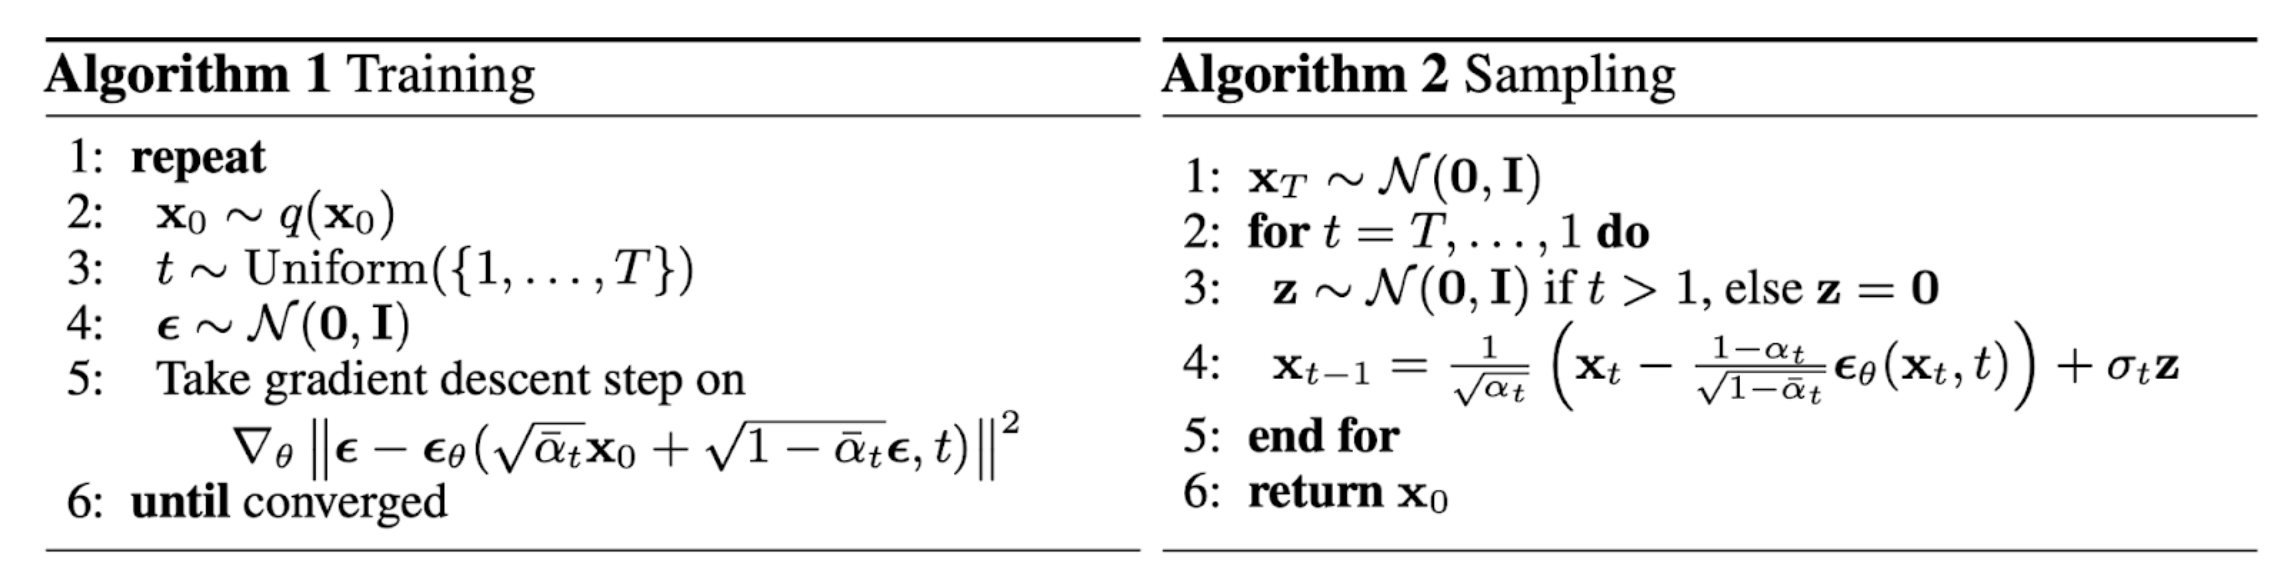
\includegraphics[scale=0.3]{image/DDPM-algo.png}
\caption{DDPM algo}
\label{fig:DDPM-algo}
\end{figure}

\section{NCSN}

% \begin{itemize}
%     \item Langevin MCMC 
%     \item  ancestral sampling
%     \item  
% \end{itemize}

% generalize  Perturbing data with multiple noise scales to infinite number of noise scales,
% 把系列离散扰动数据的分布连续化为能用随机微分方程来刻画。

% 把任意数据分布映射到先验分布(高斯分布)。

% SMLD的离散化:

% DDPM的离散化:

% 如何训练一个时间相关的分数模型:

% \begin{equation}
% \boldsymbol{\theta}^*=\underset{\boldsymbol{\theta}}{\arg \min } \mathbb{E}_t\left\{\lambda(t) \mathbb{E}_{\mathbf{x}(0)} \mathbb{E}_{\mathbf{x}(t) \mid \mathbf{x}(0)}\left[\left\|\mathbf{s}_{\boldsymbol{\theta}}(\mathbf{x}(t), t)-\nabla_{\mathbf{x}(t)} \log p_{0 t}(\mathbf{x}(t) \mid \mathbf{x}(0))\right\|_2^2\right]\right\}
% \end{equation}

% 概率流联系常微分的数值解:reverse-time SDE存在一个对应的ODE数值解法。对任意的扩散过程,存在一个确定的过程,其迹和SDE的边缘概率密度分布一致。该确定过程能用如下ODE刻画:
% \begin{equation}
% \mathbf{d} \mathbf{x}=\left[\mathbf{f}(\mathbf{x}, t)-\frac{1}{2} g(t)^2 \nabla_{\mathbf{x}} \log p_t(\mathbf{x})\right] \mathbf{d} t
% \end{equation}
% 该方程被称为:probability flow ODE。
% 该常微分方程的解迹在$t$处的采样样本的概率密度为$p_{t}(x)$。

% 令$\mathbf{f}(\mathbf{x}, t)=\mathbf{0}, g(t)=\sqrt{2t}$,(此时,$p_t(\mathbf{x})=p_{\text {data }}(\mathbf{x}) \otimes \mathcal{N}\left(\mathbf{0}, t^2 \boldsymbol{I}\right)$,其中$\otimes$表示卷积,分数模型$s_\phi(\mathbf{x}, t) \approx \nabla \log p_t(\mathbf{x})$),
% 得到 经验 PF ODE:

% \begin{equation}
% \frac{\mathbf{d} \mathbf{x}_t}{\mathbf{~d} t}=-t s_\phi\left(\mathbf{x}_t, t\right)
% \end{equation}
% $X_T$初始化,用欧拉或Heun法求解得到解迹:$\left\{\hat{\mathbf{x}}_t\right\}_{t \in[0, T]}$。$t=0$符合$p_{data}(\mathbf{x})$。 将图像映射到$[-1,1]$后,设置$T=80, s=0.002$,$s$是采样步长。

% 条件逆扩散:
% \begin{equation}
% \mathbf{d} \mathbf{x}=\left\{\mathbf{f}(\mathbf{x}, t)-g(t)^2\left[\nabla_{\mathbf{x}} \log p_t(\mathbf{x})+\nabla_{\mathbf{x}} \log p_t(\mathbf{y} \mid \mathbf{x})\right]\right\} \mathbf{d} t+g(t) \mathbf{d} \overline{\mathbf{w}}
% \end{equation}

数据样本$\left\{\mathbf{x}_i \in \mathbb{R}^D\right\}_{i=1}^N$ 满足独立同分布,数据的分布用$p_{data}(\mathbf{x})$表示,概率密度$p(\mathbf{x})$的分数定义为$\nabla_{\mathbf{x}} \log p(\mathbf{x})$,分数网络score network $s_{\theta}:\mathbb{R}^D \rightarrow \mathbb{R}^D$,其中$\theta$表示网络参数。用分数网络来刻画数据分布,因为若概率密度的分数已知,则可以利用郎之万动力采样,其采样出的数据符合数据原始分布。 因此基于分数的生成模型的核心,就是分数匹配和郎之万动力采样。

能量模型定义为:
\begin{equation}
p_m(\mathbf{x} ; \boldsymbol{\theta})=\frac{\tilde{p}_m(\mathbf{x} ; \boldsymbol{\theta})}{Z_{\boldsymbol{\theta}}}, \quad Z_{\boldsymbol{\theta}}=\int \tilde{p}_m(\mathbf{x} ; \boldsymbol{\theta}) \mathrm{d} \mathbf{x}
\end{equation}
其分数则为:
\begin{equation}
\mathbf{s}_m(\mathbf{x} ; \boldsymbol{\theta}) \triangleq \nabla_{\mathbf{x}} \log p_m(\mathbf{x} ; \boldsymbol{\theta})=\nabla_{\mathbf{x}} \log \tilde{p}_m(\mathbf{x} ; \boldsymbol{\theta}), \quad  \mathbf{s}_d(\mathbf{x} ; \boldsymbol{\theta}) \triangleq \nabla_{\mathbf{x}} \log p_d(\mathbf{x} ; \boldsymbol{\theta})
\end{equation}
消去了$Z_{\boldsymbol{\theta}}$,其中$p_d$是$p_{data}$的简写。

上述分数匹配于2005(Hyvärinen, 2005)年被提出,主要用来解决基于能量的概率密度估计(极大似然建模)分母归一化因子难处理的问题,原始优化目标为:
\begin{equation}
\frac{1}{2} \mathbb{E}_{p_{\text {data }}}\left[\left\|\mathbf{s}_{\boldsymbol{\theta}}(\mathbf{x})-\nabla_{\mathbf{x}} \log p_{\text {data }}(\mathbf{x})\right\|_2^2\right]
\end{equation}
该论文得出其等价形式:
\begin{equation}
J(\boldsymbol{\theta}) \triangleq \mathbb{E}_{p_d}\left[\operatorname{tr}\left(\nabla_{\mathbf{x}} \mathbf{s}_m(\mathbf{x} ; \boldsymbol{\theta})\right)+\frac{1}{2}\left\|\mathbf{s}_m(\mathbf{x} ; \boldsymbol{\theta})\right\|_2^2\right],
\end{equation}
其中$tr$表示矩阵的迹,上述公式需要计算 log-density的Hessian矩阵,计算量非常大。

在数学上,1981年就有了相关定理。参考数学基础部分。

Sliced Score Matching一文对(Hyvärinen, 2005)做了改进,
得出
\begin{equation}
\mathbb{E}_{p_{\mathbf{v}}} \mathbb{E}_{p_{\text {data }}}\left[\mathbf{v}^{\top} \nabla_{\mathbf{x}} \mathbf{s}_{\boldsymbol{\theta}}(\mathbf{x}) \mathbf{v}+\frac{1}{2}\left\|\mathbf{s}_{\boldsymbol{\theta}}(\mathbf{x})\right\|_2^2\right]
\end{equation}
其中$p_{\mathbf{v}}$是一个简单分布的随机向量,比如多元标准高斯分布。该结论表明,将原始高维矩阵关于随机向量做投影,去逼近式$(33)$的迹,能减少计算量的同时,保持无偏估计。

另外2010年的一篇文章A Connection Between Score Matching and Denoising Autoencoders提出的Denoising score matching能做到0梯度计算(计算量更少了)达到等价的优化效果,但是是对扰动后的数据的密度估计。具体来说,定义扰动后的数据分布为:
\begin{equation}
q_\sigma(\tilde{\mathbf{x}}) \triangleq \int q_\sigma(\tilde{\mathbf{x}} \mid \mathbf{x}) p_{\text {data }}(\mathbf{x}) \mathrm{d} \mathbf{x}
\end{equation}
于是优化目标
\begin{equation}
\frac{1}{2} \mathbb{E}_{q_\sigma(\tilde{\mathbf{x}} \mid \mathbf{x}) p_{\text {data }}(\mathbf{x})}\left[\left\|\mathbf{s}_{\boldsymbol{\theta}}(\tilde{\mathbf{x}})-\nabla_{\tilde{\mathbf{x}}} \log q_\sigma(\tilde{\mathbf{x}} \mid \mathbf{x})\right\|_2^2\right]
\end{equation}
的最优解$\mathbf{s}_{\boldsymbol{\theta}^*}(\mathbf{x})$当扰动很小的时候,有:
\begin{equation}
\mathbf{s}_{\boldsymbol{\theta}^*}(\mathbf{x})=\nabla_{\mathbf{x}} \log q_\sigma(\mathbf{x}) \approx \nabla_{\mathbf{x}} \log p_{\text {data }}(\mathbf{x})
\end{equation}

朗之万动力学在已知分数函数$\nabla_{\mathbf{x}} \log p(\mathbf{x})$的情况下,可以采样出概率密度为$p(\mathbf{x})$的样本。
具体来说:
\begin{equation}
\tilde{\mathbf{x}}_t=\tilde{\mathbf{x}}_{t-1}+\frac{\epsilon}{2} \nabla_{\mathbf{x}} \log p\left(\tilde{\mathbf{x}}_{t-1}\right)+\sqrt{\epsilon} \mathbf{z}_t
\end{equation}
其中$\epsilon$表示固定的步长大小,$\tilde{\mathbf{x}}_0 \sim \pi(\mathbf{x})$是一个先验分布,$z_t \sim \mathcal{N}(0, I)$。当$\epsilon \rightarrow 0, T \rightarrow \infty$,在一些正则条件下,$
\tilde{\mathbf{x}}_T \sim p(\mathbf{x})$。
具体分析见:
\href{https://www.stats.ox.ac.uk/~teh/research/compstats/WelTeh2011a.pdf}{Bayesian Learning via Stochastic Gradient Langevin Dynamics 2011}。

NCSN是在以上基础上提出的,作者分析了基于分数的生成模型的两个问题。基于一些基础实验,1:Sliced score matching在原始数据上的迭代损失曲线没添加噪声后的迭代平稳,而且前者是极度不平稳,上下波动很大,对此作者给出了基于流形假设的分析;2.通过分数匹配的方法,去做一个混合高斯分布的分数估计,发现在低密度区域匹配的很不准确,同时混合模型的权重因子失效严重,在混合区域,使用郎之万动力采样,是极度缓慢才能收敛到实际情况,因为分数函数关于不同混合密度的支撑集上的函数值,是和混合因子无关的,导致优化很难处理混合模型各自的连接区域的密度情况,以至于采样不准确。

基于这些基本观察,分析,作者提出了带尺度的扰动分数模型:Noise Conditional Score Networks。一来解决了高低密度不均匀难以优化,导致采样不准的问题,二来解决了数据在高维空间的低维嵌入的普遍现象导致的分数模型无法正确优化的问题。因为将数据不断扰动,能使其充满整个空间,同时,低密度区域得到了有效填充,另外不同尺度,从极小扰动到不断增幅扰动因子,使得一个分数模型在全空间中去拟合不同尺度的扰动,得到非常充分的训练,因此其逆向采样,能更好的近似到原始分布。

称$\mathbf{s}_{\boldsymbol{\theta}}(\mathbf{x}, \sigma)$为Noise Conditional Score Network (NCSN)是指:
设扰动因子$\{\sigma_i\}_{i=1}^{L}$满足$\frac{\sigma_1}{\sigma_2}=\dots=\frac{\sigma_{L-1}}{\sigma_L}>1 $,
定义扰动尺度为$\sigma$的数据分布
\begin{equation}
q_\sigma(\tilde{\mathbf{x}}) \triangleq \int p_{\text {data }}(\mathbb{t}) \mathcal{N}(\tilde{\mathbf{x}} \mid \mathbb{t}, \sigma^2I)
\end{equation}
训练一个
\begin{equation}
\forall \sigma \in\left\{\sigma_i\right\}_{i=1}^L: \mathbf{s}_{\boldsymbol{\theta}}(\tilde{\mathbf{x}}, \sigma) \approx \nabla_{\mathbf{x}} \log q_\sigma(\tilde{\mathbf{x}})
\end{equation}
的网络,其中$ \mathbf{x} \in \mathbb{R}^{D}, \mathbf{s}_{\boldsymbol{\theta}} \in \mathbb{R}^{D}$。

因$q_\sigma(\tilde{\mathbf{x}} \mid \mathbf{x})=\mathcal{N}\left(\tilde{\mathbf{x}} \mid \mathbf{x}, \sigma^2 I\right)$,有$\nabla_{\tilde{\mathbf{x}}} \log q_\sigma(\tilde{\mathbf{x}} \mid \mathbf{x})=-(\tilde{\mathbf{x}}-\mathbf{x}) / \sigma^2$,于是对于给定的尺度$\sigma$,其去噪分数匹配损失为:
\begin{equation}
\ell(\boldsymbol{\theta} ; \sigma) \triangleq \frac{1}{2} \mathbb{E}_{p_{\text {data }}(\mathbf{x})} \mathbb{E}_{\tilde{\mathbf{x}} \sim \mathcal{N}\left(\mathbf{x}, \sigma^2 I\right)}\left[\left\|\mathrm{s}_{\boldsymbol{\theta}}(\tilde{\mathbf{x}}, \sigma)+\frac{\tilde{\mathbf{x}}-\mathrm{x}}{\sigma^2}\right\|_2^2\right]
\end{equation}
对于所有尺度$\forall \sigma \in\left\{\sigma_i\right\}_{i=1}^L$得到最终的优化目标:
\begin{equation}
\mathcal{L}\left(\boldsymbol{\theta} ;\left\{\sigma_i\right\}_{i=1}^L\right) \triangleq \frac{1}{L} \sum_{i=1}^L \lambda\left(\sigma_i\right) \ell\left(\boldsymbol{\theta} ; \sigma_i\right)
\end{equation}其中$ \lambda\left(\sigma_i\right)>0$,为依赖于$\sigma_i$的系数函数。

该目标函数的最优解$\mathbf{s}_{\boldsymbol{\theta}^*}(\mathbf{x}, \sigma)$满足
$\forall i \in \{1, 2, \cdots, L \}, \mathbf{s}_{\boldsymbol{\theta}^*}\left(\mathbf{x}, \sigma_i\right)=\nabla_{\mathbf{x}} \log q_{\sigma_i}(\mathbf{x})$。$\lambda(\cdot)$选择使得所有尺度因子的数量级一致,经验得知,一个训练好的分数模型,其范数正比于尺度的倒数,又$\frac{\tilde{\mathbf{x}}-\mathbf{x}}{\sigma} \sim \mathcal{N}(0, I)$,因此,选择$\lambda(\sigma)=\sigma^2$,使得$\left\|\sigma \mathbf{s}_{\boldsymbol{\theta}}(\mathbf{x}, \sigma)\right\|_2 \propto 1$。

最后论文提出了annealed Langevin dynamics采样算法(对比式(38)):
将原始步长$\epsilon$改进为$\epsilon \cdot \sigma^2_i / \sigma^2_L$。
\begin{figure}[h!]
\centering
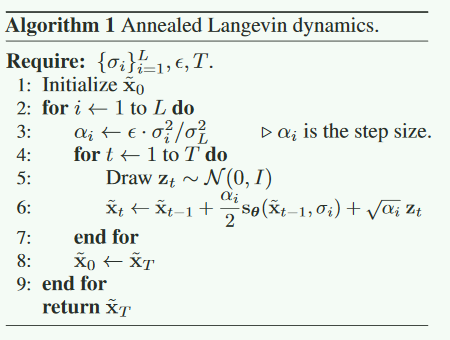
\includegraphics[scale=0.9]{image/NCSNLD.jpg}
\caption{NCSN annealed Langevin dynamics}
\label{fig:NCSN}
\end{figure}

\subsection{score matching}

\subsection{极大似然的计算}
Yang Song继其SGM模型,给出了SDE解的边缘分布同数据的分布的KL散度与SM模型优化对象的存在一个不等关系,使得优化SM模型,能得到SDE对应的数据边缘分布,也就是原始数据的似然函数值。

具体来讲:
\begin{equation}
D_{\mathrm{KL}}\left(p \| p_{\boldsymbol{\theta}}^{\mathrm{SDE}}\right) \leq \mathcal{J}_{\mathrm{SM}}\left(\boldsymbol{\theta} ; g(\cdot)^2\right)+D_{\mathrm{KL}}\left(p_T \| \pi\right)
\end{equation}
论文的网络是使用概率流网络来训练的?。

在此基础上Cheng Lu等人,给出了扩散对应的ODE的似然函数的上界。
\begin{equation}
\mathcal{J}_{\mathrm{ODE}}(\theta) \leq \sqrt{\mathcal{J}_{\mathrm{SM}}(\theta)} \cdot \sqrt{\mathcal{J}_{\text {Fisher }}(\theta)}
\end{equation}

论文证明了一阶分数模型并不能得到扩散对应的ODE的似然,该似然被一阶,二阶,三阶分数匹配误差所控制,以此提出了一个高阶的分数去噪模型,能得到更好的原始数据的似然逼近,并同时能保证生成高质量数据。

\section{连续版Score SDE}
SDE中的噪声尺度因子,和NCSN的写法就大小比较在指标上是相反的,原因在于使用DDPM的方式,重新定义了NCSN中的优化目标,得到
\begin{equation}
\boldsymbol{\theta}^*=\underset{\boldsymbol{\theta}}{\arg \min } \sum_{i=1}^N\left(1-\alpha_i\right) \mathbb{E}_{p_{\text {data }}(\mathbf{x})} \mathbb{E}_{p_{\alpha_i}(\tilde{\mathbf{x}} \mid \mathbf{x})}\left[\left\|\mathbf{s}_{\boldsymbol{\theta}}(\tilde{\mathbf{x}}, i)-\nabla_{\tilde{\mathbf{x}}} \log p_{\alpha_i}(\tilde{\mathbf{x}} \mid \mathbf{x})\right\|_2^2\right] .
\end{equation}
和逆向马尔科夫链(采样)
\begin{equation}
\mathbf{x}_{i-1}=\frac{1}{\sqrt{1-\beta_i}}\left(\mathbf{x}_i+\beta_i \mathbf{s}_{\boldsymbol{\theta}^*}\left(\mathbf{x}_i, i\right)\right)+\sqrt{\beta_i} \mathbf{z}_i, \quad i=N, N-1, \cdots, 1
\end{equation}
论文中将其称为ancestral sampling。

问题是(43)式能通过ELBO推导出来?通过ELBO推导出来,优化的是均值,而转移概率为高斯,对数求导后,差不多也是均值。仔细检查下,应该就是通过ELBO得到(43)所示的分数表达形式。

两者的分数表达形式和采样形式差别不大,将其连续化,并做形式上的推广,得到$It\hat{o}$ SDE方程:
\begin{equation}
\mathrm{d} \mathbf{x}=\mathbf{f}(\mathbf{x}, t) \mathrm{d} t+g(t) \mathrm{d} \mathbf{w}
\end{equation}
而Anderson (1982) 的论文表示,其逆向也是扩散过程, reverse-time SDE为:
\begin{equation}
\mathrm{d} \mathbf{x}=\left[\mathbf{f}(\mathbf{x}, t)-g(t)^2 \nabla_{\mathbf{x}} \log p_t(\mathbf{x})\right] \mathrm{d} t+g(t) \mathrm{d} \overline{\mathbf{w}}
\end{equation}
其对应的优化目标可写为:
\begin{equation}
\boldsymbol{\theta}^*=\underset{\boldsymbol{\theta}}{\arg \min } \mathbb{E}_t\left\{\lambda(t) \mathbb{E}_{\mathbf{x}(0)} \mathbb{E}_{\mathbf{x}(t) \mid \mathbf{x}(0)}\left[\left\|\mathbf{s}_{\boldsymbol{\theta}}(\mathbf{x}(t), t)-\nabla_{\mathbf{x}(t)} \log p_{0 t}(\mathbf{x}(t) \mid \mathbf{x}(0))\right\|_2^2\right]\right\} .
\end{equation}
其中$\lambda:[0, T] \rightarrow \mathbb{R}_{>0}, t\in [0, T], \mathbf{x}(0) \sim p_0(\mathbf{x}), \mathbf{x}_t \sim p_{0t}(\mathbf{x}(t) \mid \mathbf{x}(0))$
其解$\mathbf{s}_{\boldsymbol{\theta}^*}\left(\mathbf{x}, t\right)=\nabla_{\mathbf{x}} \log p_{t}(\mathbf{x})$对几乎所有$\mathbf{x}, t$成立。
另外需要注意的是,当转移核是优化目标(47)的解的时候,若$\mathbf{f}(\cdot, t)$是仿射的,则转移核是高斯分布。均值和方程能具体计算出来,参考( Arno Solin 2019)Applied stochastic differential equations。

这里需要注意的是,论文2.1节指出,NCSN尺度上的逆向描述被简写为SMLD(DENOISING SCORE MATCHING WITH LANGEVIN  DYNAMICS),另外在3.4节,对其做连续化SDE推导的时候,扩散过程也是满足马尔可夫性的。这点和NCSN中从大到小尺度添加噪声训练分数匹配模型NCSN是不同的,其扰动核没有马尔可夫性假设,但是蕴含了马尔科夫性。
具体来说,$p_{\sigma_i}(\mathbf{x} \mid \mathbf{x_0})$对应的$\mathbf{x}_i$满足如下的马尔科夫链:
\begin{equation}
\mathbf{x}_i=\mathbf{x}_{i-1}+\sqrt{\sigma_i^2-\sigma_{i-1}^2} \mathbf{z}_{i-1}, \quad i=1, \cdots, N
\end{equation}
这里方差是$\sigma_i^2-\sigma_{i-1}^2$的原因在于SMLD并不是DDPM那样递归的定义,而是在$\mathbf{x}_0$上,逐级的增加扰动噪声$\mathbf{x}_{\sigma_i}=\mathbf{x}_0+\sigma_i \mathbf{I}$。上式连续化得到
\begin{equation}
\mathrm{d} \mathbf{x}=\sqrt{\frac{\mathrm{d}\left[\sigma^2(t)\right]}{\mathrm{d} t}} \mathrm{~d} \mathbf{w} .
\end{equation}
表达了$\{\mathbf{x}(t)\}^{1}_{t=0}$的前向过程的SDE形式。

DDPM的扰动核$\left\{p_{\alpha_i}\left(\mathbf{x} \mid \mathbf{x}_0\right)\right\}_{i=1}^N$
对应的离散马尔科夫链:
\begin{equation}
\mathbf{x}_i=\sqrt{1-\beta_i} \mathbf{x}_{i-1}+\sqrt{\beta_i} \mathbf{z}_{i-1}, \quad i=1, \cdots, N
\end{equation}
当$N \rightarrow \infty$时,收敛到如下SDE:

\begin{equation}
\mathrm{d} \mathbf{x}=-\frac{1}{2} \beta(t) \mathbf{x} \mathrm{d} t+\sqrt{\beta(t)} \mathrm{d} \mathbf{w}
\end{equation}

论文称SMLD的SDE为Variance Exploding (VE) SDE, 称DDPM的SDE为Variance Preserving (VP) SDE, 并给出了 sub-VP SDE:
\begin{equation}
\mathrm{d} \mathbf{x}=-\frac{1}{2} \beta(t) \mathbf{x} \mathrm{d} t+\sqrt{\beta(t)\left(1-e^{-2 \int_0^t \beta(s) \mathrm{d} s}\right)} \mathrm{d} \mathbf{w}
\end{equation}其在似然函数的计算上更加准确。

当得到分数模型后,就可以利用reverse-time SDE 采样得到生成样本。数值求解器也可以提供来自SDEs的近似轨迹,比如Euler-Maruyama,Runge-Kutta methods等方法,可以用来求解reverse-time SDE,获得生成样本。
另外DDPM的祖先采样法,不能用在VE SDE,作者这里提出了reverse diffusion samplers,具体分析细节可看附录E部分。因为这里有训练好的分数模型,有利于求解,而分数模型有对应的郎之万MCMC采样,因此作者综合考虑这些特性,给出了Predictor-Corrector(PC) samplers 采样器,其结合了分数模型的采样特点,也考虑了SDE的数值求解,同时也考虑了DDPM等的采样方法。
细节见附录部分。
\begin{figure}[h!]
\centering
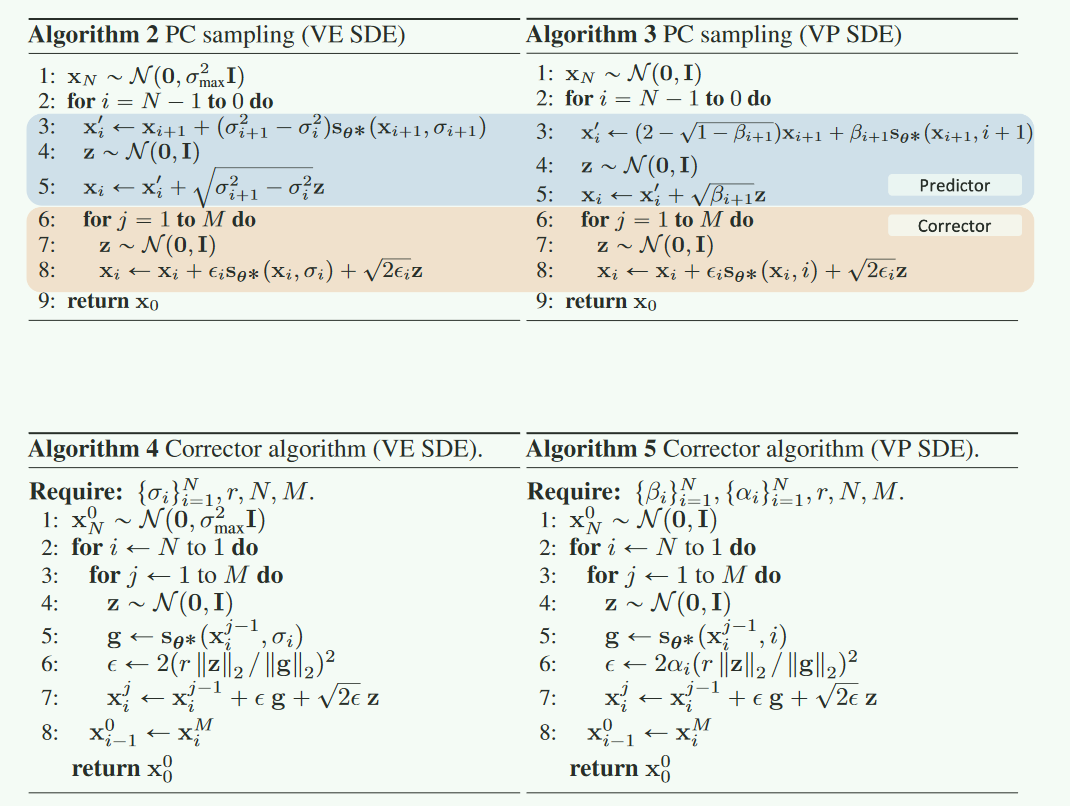
\includegraphics[scale=0.5]{image/PredictorCorrector.jpg}
\caption{SDE Predictor Corrector}
\label{fig:PC}
\end{figure}

另外SDE有对应的常微分方程,
\begin{equation}
\mathrm{d} \mathbf{x}=\left[\mathbf{f}(\mathbf{x}, t)-\frac{1}{2} g(t)^2 \nabla_{\mathbf{x}} \log p_t(\mathbf{x})\right] \mathrm{d} t
\end{equation}
该常微分方程的解,保持SDE所有边缘分布,且构成是确定的。作者将其称为probability flow ODE。当分析模型得到恰当的训练后,它就是一个neural network(Neural Ordinary Differential Equations),且能用来精确的计算数据(在量化的意义下)的似然值。这块内容在“极大似然的计算”章节中细讲。
% \subsection{stochastic gradient Langevin dynamics}

\section{一些理论结果}

\section{采样加速}
\subsection{DDIM}
将DDPM的前向马尔科夫链推广为非马尔科夫过程。
$$
q_\sigma\left(x_{1: T} \mid x_0\right):=q_\sigma\left(x_T \mid x_0\right) \prod_{t=2}^T q_\sigma\left(x_{t-1} \mid x_t, x_0\right)
$$
where $q_\sigma\left(\boldsymbol{x}_T \mid \boldsymbol{x}_0\right)=\mathcal{N}\left(\sqrt{\alpha_T} \boldsymbol{x}_0,\left(1-\alpha_T\right) \boldsymbol{I}\right)$ and for all $t>1$,
$$
q_\sigma\left(x_{t-1} \mid x_t, x_0\right)=\mathcal{N}\left(\sqrt{\alpha_{t-1}} x_0+\sqrt{1-\alpha_{t-1}-\sigma_t^2} \cdot \frac{x_t-\sqrt{\alpha_t} x_0}{\sqrt{1-\alpha_t}}, \sigma_t^2 \boldsymbol{I}\right) .
$$

The mean function is chosen to order to ensure that $q_\sigma\left(x_t \mid x_0\right)=\mathcal{N}\left(\sqrt{\alpha_t} x_0,\left(1-\alpha_t\right) \boldsymbol{I}\right)$ for all $t$ (see Lemma 1 of Appendix B), so that it defines a joint 
inference distribution that matches the "marginals" as desired. The forward process ${ }^3$ can be derived from Bayes' rule:
$$
q_\sigma\left(x_t \mid x_{t-1}, x_0\right)=\frac{q_\sigma\left(x_{t-1} \mid x_t, x_0\right) q_\sigma\left(x_t \mid x_0\right)}{q_\sigma\left(x_{t-1} \mid x_0\right)}
$$
因为这篇文章是在SGM之后,所以也做了ODE的分析。推导过程和ELBO一致,不赘述。

后续文章ANALYTIC-DPM证明了DDPM,DDIM论文中轨迹中的最优均值和最优方差,均可解析解到,但是,解是用分数函数来表达的,其实就相当于没有,因为分数模型的训练就是DDPM模型的训练。ANALYTIC-DPM一文的前向是DDIM的模式,但是在推导过程中,作者把均值用DDIM模型表达的式子替换为理论上等价的分数模型,因分数模型有具体的表达式,因此整个计算能走下去。

\subsection{ODE求解:dpm++等}
DPM-Solver是用SDE的思路,写出DDPM的reverse time SDE 和diffusion  ODE,并利用变量替换法,给出了ODE的具体解,具体解的形式在ODE的数值求解中有充分的研究,因此能避免成百次的迭代,达到加速的效果。

DPM-Solver++是在DPM-Solver的基础上,考虑了引导因子(guide scale)$s$,并在多阶展开逼近上,给出了较DPM-Solver更具体的多阶求解器,同时证明了DDIM是其一阶求解器。另外考虑引导因子,是因为扩散模型训练中发现增加分类引导(calssify-free guide),能带来更好的生成效果。

因为算法本身和训练无关,只用在采样生成样本中,因此法只需要不多的代码,就能实现,而且在实际中成为比较好的加速版的采样求解器。
\subsection{蒸馏}


\section{一致性模型}
PF ODE将数据光滑的映射到噪声,一致性模型将ODE的迹上的任意点$x_{t^{\prime}}, x_T$映射到初始点$x_0$。这些所有映射被称为一致性模型,因为其在一个迹上的输出都被映射到迹中初始点了。 A notable property of our model is self-consistency: points on the same trajectory map to the same initial point.

这里的一致性主要为了加速采样的。
两种训练方式:需要一个扩散模型+对应的ODE,在PF ODE的迹上生成成对的相邻点。最小化这些成对点关于模型的输出的差(L1/L2)值。二种方式是单独训练一致性模型。
蒸馏训练:

$$\begin{aligned} & \mathcal{L}_{C D}^N\left(\boldsymbol{\theta}, \boldsymbol{\theta}^{-} ; \boldsymbol{\phi}\right):= \\ & \quad \mathbb{E}\left[\lambda\left(t_n\right) d\left(\boldsymbol{f}_{\boldsymbol{\theta}}\left(\mathbf{x}_{t_{n+1}}, t_{n+1}\right), \boldsymbol{f}_{\boldsymbol{\theta}^{-}}\left(\hat{\mathbf{x}}_{t_n}^\phi, t_n\right)\right)\right]\end{aligned}$$

蒸馏方式可以将扩散模型蒸馏到一次采样。

独立训练基础:

$\text { Lemma 1. Let } \mathbf{x} \sim p_{\text {data }}(\mathbf{x}), \mathbf{x}_t \sim \mathcal{N}\left(\mathbf{x} ; t^2 \boldsymbol{I}\right)$ \text {, and }  $p_t\left(\mathbf{x}_t\right)=p_{\text {data }}(\mathbf{x}) \otimes \mathcal{N}\left(\mathbf{0}, t^2 \boldsymbol{I}\right) $ \text {. We have } 
\begin{equation} 
  \nabla \log p_t(\mathbf{x})=-\mathbb{E}\left[\frac{\mathbf{x}_t-\mathbf{x}}{t^2} \mid \mathbf{x}_t\right] \text {. }
\end{equation}

一个随便的网络作为一致性函数的逼近表达:
$\boldsymbol{f}_{\boldsymbol{\theta}}(\mathbf{x}, t)=c_{\text {skip }}(t) \mathbf{x}+c_{\text {out }}(t) F_{\boldsymbol{\theta}}(\mathbf{x}, t)$

\subsection{LCM}
自编码$(\mathcal{E}, \mathcal{D})$:$z=\mathcal{E}(x), \bar{x}=\mathcal{D}(z)$将图像压缩到隐变量空间,在隐变量空间中,逆向扩散过程的PF-ODE为:
\begin{equation}
\frac{\mathbf{d} \boldsymbol{z}_t}{\mathbf{~d} t}=f(t) \boldsymbol{z}_t+\frac{g^2(t)}{2 \sigma_t} \boldsymbol{\epsilon}_\theta\left(\boldsymbol{z}_t, \boldsymbol{c}, t\right), \quad \boldsymbol{z}_T \sim \mathcal{N}\left(\mathbf{0}, \tilde{\sigma}^2 \boldsymbol{I}\right)
\end{equation}
其中$\boldsymbol{\epsilon}_\theta\left(\boldsymbol{z}_t, \boldsymbol{c}, t\right)$表示噪声预测模型,$\boldsymbol{c}$是条件因子,比如文本。

定义一致性函数:$f_{\boldsymbol{\theta}}:\left(z_{\boldsymbol{t}}, \boldsymbol{c}, t\right) \mapsto z_0$

\begin{equation}
\boldsymbol{f}_{\boldsymbol{\theta}}(\boldsymbol{z}, \boldsymbol{c}, t)=c_{\text {skip }}(t) \boldsymbol{z}+c_{\mathbf{out}}(t)\left(\frac{\boldsymbol{z}-\sigma_t \hat{\boldsymbol{\epsilon}}_\theta(\boldsymbol{z}, \boldsymbol{c}, t)}{\alpha_t}\right)
\end{equation}
其中$c_{skip}(0)=1, c_{skip}(0)=0$, $\boldsymbol{\bar{\epsilon}}_\theta\left(\boldsymbol{z}_t, \boldsymbol{c}, t\right)$ 为一预训练扩散模型作为初始化的网络。

这里常微分的边缘解,用了DPM++这种数值解方式。
容易给出一致性蒸馏损失:
\begin{equation}
\mathcal{L}_{\mathcal{C D}}\left(\boldsymbol{\theta}, \boldsymbol{\theta}^{-} ; \Psi\right)=\mathbb{E}_{\boldsymbol{z}, \boldsymbol{c}, n}\left[d\left(\boldsymbol{f}_{\boldsymbol{\theta}}\left(\boldsymbol{z}_{t_{n+1}}, \boldsymbol{c}, t_{n+1}\right), \boldsymbol{f}_{\boldsymbol{\theta}^{-}}\left(\hat{\boldsymbol{z}}_{t_n}^{\Psi}, \boldsymbol{c}, t_n\right)\right)\right]
\end{equation}

其中$\hat{\boldsymbol{z}}_{t_n}^{\Psi}$表示使用ODE解$\Psi$ 从$t_{n+1} \rightarrow t_n$:
\begin{equation}
\hat{z}_{t_n}^{\Psi}-z_{t_{n+1}}=\int_{t_{n+1}}^{t_n}\left(f(t) z_t+\frac{g^2(t)}{2 \sigma_t} \epsilon_\theta\left(z_t, \boldsymbol{c}, t\right)\right) \mathbf{d} t \approx \Psi\left(z_{t_{n+1}}, t_{n+1}, t_n, \boldsymbol{c}\right)
\end{equation}

增加CFG对文字图像对齐,以及生成质量提高都能带来好处, 在原始扩散模型中,CFG使用如下:
\begin{equation}
\tilde{\boldsymbol{\epsilon}}_\theta\left(z_t, \omega, \boldsymbol{c}, t\right):=(1+\omega) \boldsymbol{\epsilon}_\theta\left(z_t, \boldsymbol{c}, t\right)-\omega \boldsymbol{\epsilon}_\theta\left(z_t, \varnothing, t\right)
\end{equation}
其中$\omega$称为guidance scale。
将此式作为替换项即可。
同时为了能使用DDIM, DPM++来解PF-ODE, 对替换后的式子需做如下简化:
\begin{equation}
\begin{aligned}
\hat{\boldsymbol{z}}_{t_n}^{\Psi, \omega}-\boldsymbol{z}_{t_{n+1}} & =\int_{t_{n+1}}^{t_n}\left(f(t) \boldsymbol{z}_t+\frac{g^2(t)}{2 \sigma_t} \tilde{\boldsymbol{\epsilon}}_\theta\left(\boldsymbol{z}_t, \omega, \boldsymbol{c}, t\right)\right) \mathbf{d} t \\
& =(1+\omega) \int_{t_{n+1}}^{t_n}\left(f(t) \boldsymbol{z}_t+\frac{g^2(t)}{2 \sigma_t} \boldsymbol{\epsilon}_\theta\left(\boldsymbol{z}_t, \boldsymbol{c}, t\right)\right) \mathbf{d} t-
\omega \int_{t_{n+1}}^{t_n}\left(f(t) \boldsymbol{z}_t+\frac{g^2(t)}{2 \sigma_t} \boldsymbol{\epsilon}_\theta\left(\boldsymbol{z}_t, \varnothing, t\right)\right) \mathbf{d} t \\
& \approx(1+\omega) \Psi\left(\boldsymbol{z}_{t_{n+1}}, t_{n+1}, t_n, \boldsymbol{c}\right)-\omega \Psi\left(\boldsymbol{z}_{t_{n+1}}, t_{n+1}, t_n, \varnothing\right) .
\end{aligned}
\end{equation}

\begin{figure}[h!]
\centering
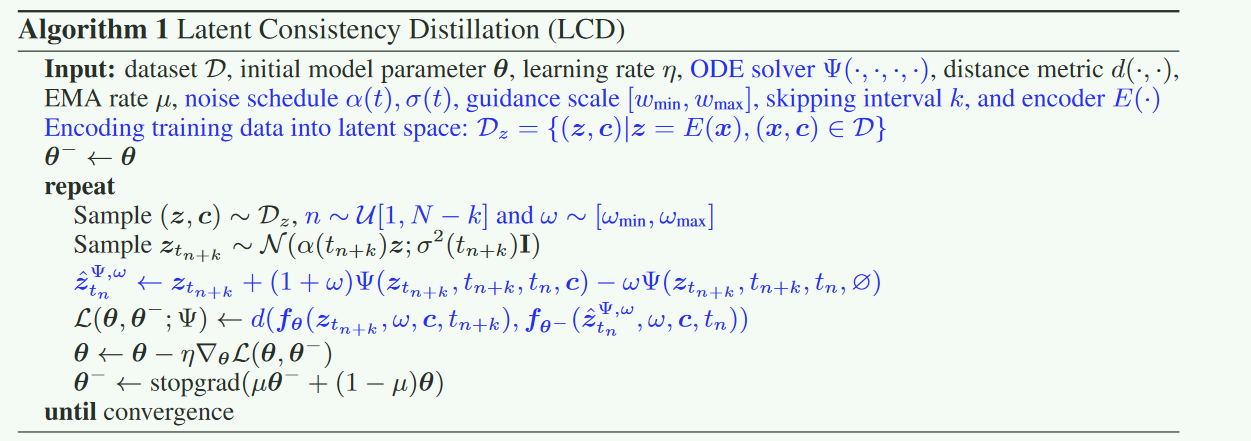
\includegraphics[scale=0.7]{image/LCD.jpg}
\caption{Latent Consistency Distillation}
\label{fig:LCD}
\end{figure}

\subsection{角色一致性}

\section{应用}
\begin{itemize}
    \item 1千万文本对数据,模型参数22M :DeepSpeed ZeRO-2 +  8 V100 + 1M steps + bs=8 per GPU
    \item 5千万图文对+1千万高质量人数据:48 NVIDIA H800 GPUs (80GB) + 2 per GPU ( InstantID)
    \item 3百万图文对数据,模型参数1431.6M(367M): 10 epochs using 8 Tesla A100 GPUs+progressive 
    \item 百万数据+万ID+caption:8 A100 GPUs + two weeks + bs=48
    \item 256-coreTPU-v3 pod, training DiT-L takes 12 hours.
    \item 通常是128*60=48*180:沉没成本比较大
    \item 组合思路难度小,混杂的库太多,数据集制作繁杂,比较占资源(意义不大)
    \item 优点:1d 扩散,simplify unet, only one bvh(400+frames) data, any topology,  4GGPU memory, 1 hour training cost, 5 infer applications,long frames generator
\end{itemize}

\subsection{多模态}

排列组合+卡+数据,太多了。

\subsubsection{VAE、CLIP、U-Net、U-ViT等模块}
\subsubsection{条件控制}

\subsection{变大}
\subsubsection{SDXL}
\subsection{Finetune}
\subsubsection{LORA}
\subsection{3D重建}
\subsection{动画动作生成}
\subsubsection{SinMDM}

\section{框架实现}
\subsection{Diffusers、SCEPTER}
\subsection{ComfyUI、WebUI、Fooocus}


\chapter{部署}
\section{量化}
\section{TensorRTt}
\section{TritonServer}
\section{OneDiff}

\chapter{商业}
\section{Sora}

% $q\left(\mathbf{x}_{1: T} \mid \mathbf{x}_0\right)=\prod_{t=1}^T q\left(\mathbf{x}_t \mid \mathbf{x}_{t-1}\right)$



\chapter{ElegantBook 写作示例}

\begin{introduction}
  \item 积分定义~\ref{def:int}
  \item Fubini 定理~\ref{thm:fubi}
  \item 最优性原理~\ref{pro:max}
  \item 柯西列性质~\ref{property:cauchy}
  \item 韦达定理
\end{introduction}

\section{Lebesgue 积分}
在前面各章做了必要的准备后,本章开始介绍新的积分。在 Lebesgue 测度理论的基础上建立了 Lebesgue 积分,其被积函数和积分域更一般,可以对有界函数和无界函数统一处理。正是由于 Lebesgue 积分的这些特点,使得 Lebesgue 积分比 Riemann 积分具有在更一般条件下的极限定理和累次积分交换积分顺序的定理,这使得 Lebesgue 积分不仅在理论上更完善,而且在计算上更灵活有效。

Lebesgue 积分有几种不同的定义方式。我们将采用逐步定义非负简单函数,非负可测函数和一般可测函数积分的方式。

由于现代数学的许多分支如概率论、泛函分析、调和分析等常常用到一般空间上的测度与积分理论,在本章最后一节将介绍一般的测度空间上的积分。

\subsection{积分的定义}

我们将通过三个步骤定义可测函数的积分。首先定义非负简单函数的积分。以下设 $E$ 是 $\mathcal{R}^n$ 中的可测集。

\begin{definition}[可积性] \label{def:int} 
设 $ f(x)=\sum\limits_{i=1}^{k} a_i \chi_{A_i}(x)$ 是 $E$ 上的\textbf{非负简单函数},中文其中 $\{A_1,A_2,\ldots,A_k\}$ 是 $E$ 上的一个可测分割,$a_1,a_2,\ldots,a_k$ 是非负实数。定义 $f$ 在 $E$ 上的积分为 $\int_{a}^b f(x)$
\begin{equation}
   \label{inter}
   \int_{E} f dx = \sum_{i=1}^k a_i m(A_i) \pi \alpha\beta\sigma\gamma\nu\xi\epsilon\varepsilon. \oint_{a}^b\ointop_{a}^b\prod_{i=1}^n
\end{equation}
一般情况下 $0 \leq \int_{E} f dx \leq \infty$。若 $\int_{E} f dx < \infty$,则称 $f$ 在 $E$ 上可积。
\end{definition}

一个自然的问题是,Lebesgue 积分与我们所熟悉的 Riemann 积分有什么联系和区别?在 4.4 在我们将详细讨论 Riemann 积分与 Lebesgue 积分的关系。这里只看一个简单的例子。设 $D(x)$ 是区间 $[0,1]$ 上的 Dirichlet 函数。即 $D(x)=\chi_{Q_0}(x)$,其中 $Q_0$ 表示 $[0,1]$ 中的有理数的全体。根据非负简单函数积分的定义,$D(x)$ 在 $[0,1]$ 上的 Lebesgue 积分为
\begin{equation}
   \label{inter2}
   \int_0^1 D(x)dx = \int_0^1 \chi_{Q_0} (x) dx = m(Q_0) = 0
\end{equation}
即 $D(x)$ 在 $[0,1]$ 上是 Lebesgue 可积的并且积分值为零。但 $D(x)$ 在 $[0,1]$ 上不是 Riemann 可积的。


有界变差函数是与单调函数有密切联系的一类函数。有界变差函数可以表示为两个单调递增函数之差。与单调函数一样,有界变差函数几乎处处可导。与单调函数不同,有界变差函数类对线性运算是封闭的,它们构成一线空间。练习题 \ref{exer:43} 是一个性质的证明。

\begin{exercise}\label{exer:43}
设 $f \notin\in L(\mathcal{R}^1)$,$g$ 是 $\mathcal{R}^1$ 上的有界可测函数。证明函数
\begin{equation}
   \label{ex:1}
   I(t) = \int_{\mathcal{R}^1} f(x+t)g(x)dx \quad t \in \mathcal{R}^1
\end{equation}
是 $\mathcal{R}^1$ 上的连续函数。 
\end{exercise}

\begin{solution}
即 $D(x)$ 在 $[0,1]$ 上是 Lebesgue 可积的并且积分值为零。但 $D(x)$ 在 $[0,1]$ 上不是 Riemann 可积的。
\end{solution}

\begin{proof}
即 $D(x)$ 在 $[0,1]$ 上是 Lebesgue 可积的并且积分值为零。但 $D(x)$ 在 $[0,1]$ 上不是 Riemann 可积的。
\end{proof}

\begin{theorem}[Fubini 定理] \label{thm:fubi} 
(1)若 $f(x,y)$ 是 $\mathcal{R}^p\times\mathcal{R}^q$ 上的非负可测函数,则对几乎处处的 $x\in \mathcal{R}^p$,$f(x,y)$ 作为 $y$ 的函数是 $\mathcal{R}^q$ 上的非负可测函数,$g(x)=\int_{\mathcal{R}^q}f(x,y) dy$ 是 $\mathcal{R}^p$ 上的非负可测函数。并且
\begin{equation}
   \label{eq:461}
   \int_{\mathcal{R}^p\times\mathcal{R}^q} f(x,y) dxdy=\int_{\mathcal{R}^p}\left(\int_{\mathcal{R}^q}f(x,y)dy\right)dx.
\end{equation}

(2)若 $f(x,y)$ 是 $\mathcal{R}^p\times\mathcal{R}^q$ 上的可积函数,则对几乎处处的 $x\in\mathcal{R}^p$,$f(x,y)$ 作为 $y$ 的函数是 $\mathcal{R}^q$ 上的可积函数,并且 $g(x)=\int_{\mathcal{R}^q}f(x,y) dy$ 是 $\mathcal{R}^p$ 上的可积函数。而且~\eqref{eq:461} 成立。
\end{theorem}

\begin{note}
在本模板中,引理(lemma),推论(corollary)的样式和定理~\ref{thm:fubi} 的样式一致,包括颜色,仅仅只有计数器的设置不一样。
\end{note}

我们说一个实变或者复变量的实值或者复值函数是在区间上平方可积的,如果其绝对值的平方在该区间上的积分是有限的。所有在勒贝格积分意义下平方可积的可测函数构成一个希尔伯特空间,也就是所谓的 $L^2$ 空间,几乎处处相等的函数归为同一等价类。形式上,$L^2$ 是平方可积函数的空间和几乎处处为 0 的函数空间的商空间。

\begin{proposition}[最优性原理] \label{pro:max}
如果 $u^*$ 在 $[s,T]$ 上为最优解,则 $u^*$ 在 $[s, T]$ 任意子区间都是最优解,假设区间为 $[t_0, t_1]$ 的最优解为 $u^*$ ,则 $u(t_0)=u^{*}(t_0)$,即初始条件必须还是在 $u^*$ 上。
\end{proposition}

我们知道最小二乘法可以用来处理一组数据,可以从一组测定的数据中寻求变量之间的依赖关系,这种函数关系称为经验公式。本课题将介绍最小二乘法的精确定义及如何寻求点与点之间近似成线性关系时的经验公式。假定实验测得变量之间的 $n$ 个数据,则在平面上,可以得到 $n$ 个点,这种图形称为 “散点图”,从图中可以粗略看出这些点大致散落在某直线近旁, 我们认为其近似为一线性函数,下面介绍求解步骤。

\begin{figure}[htbp]
  \centering
  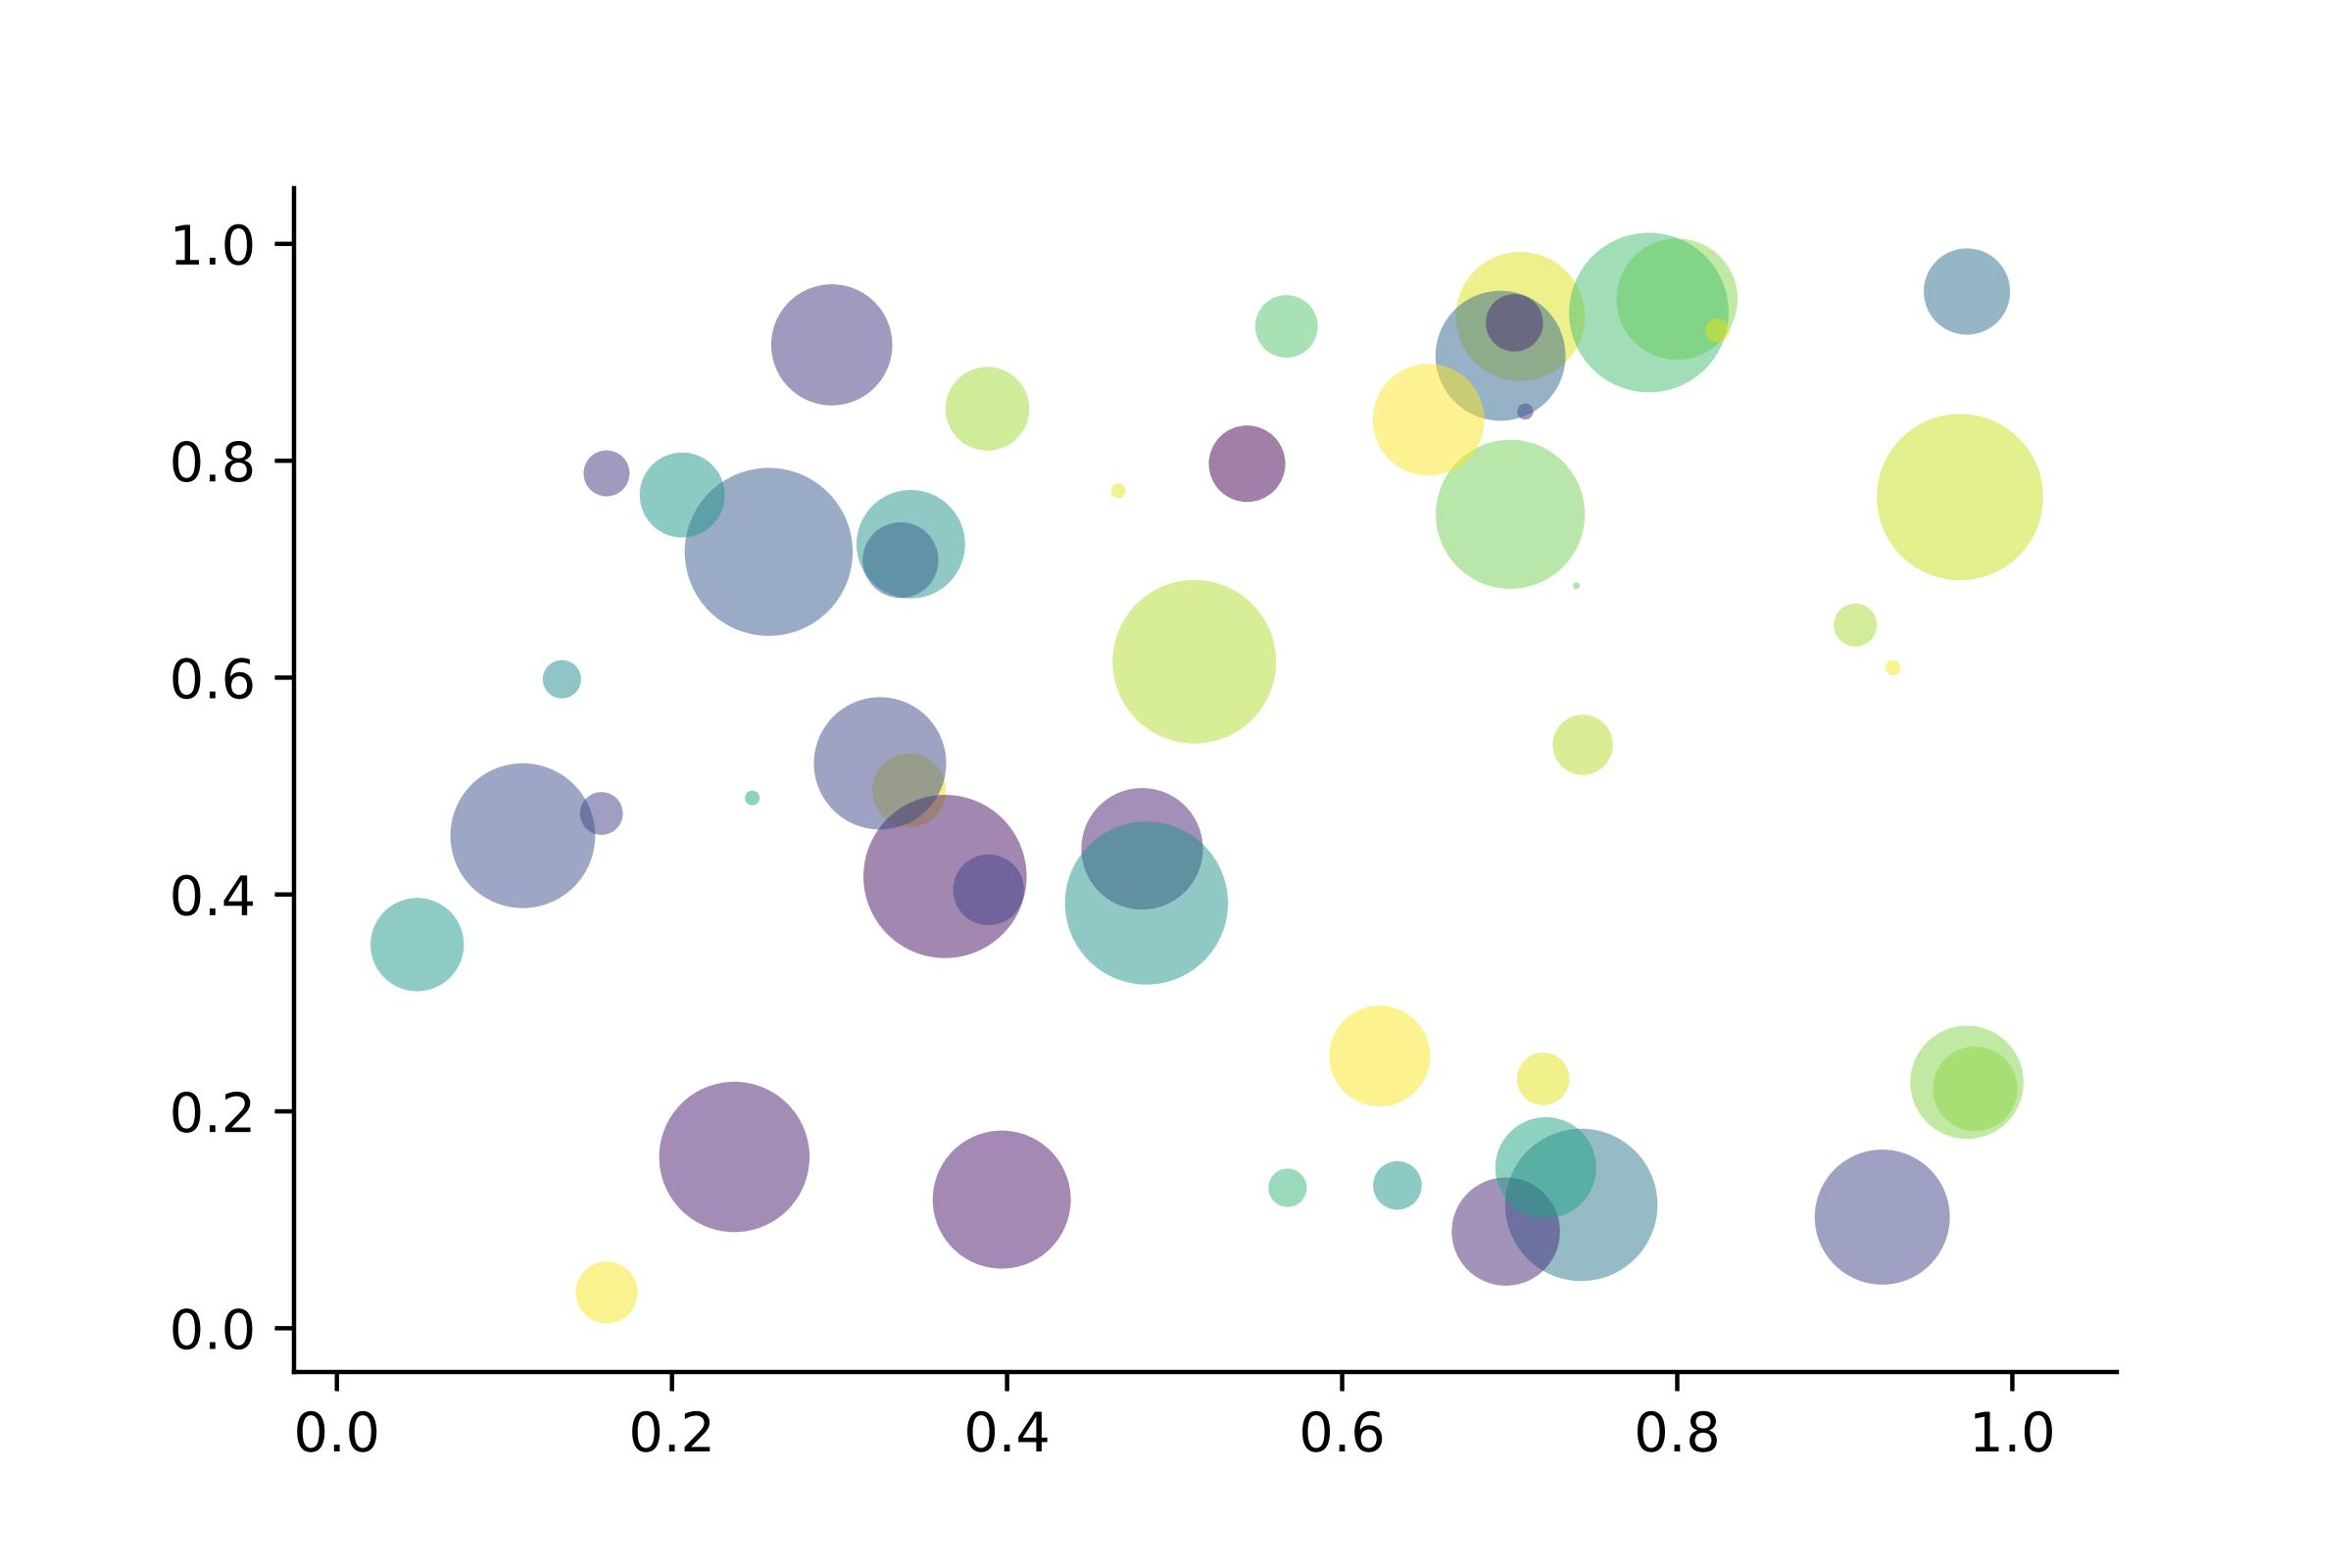
\includegraphics[width=0.6\textwidth]{image/scatter.jpg}
  \caption{散点图示例 $\hat{y}=a+bx$ \label{fig:scatter}}
\end{figure}

以最简单的一元线性模型来解释最小二乘法。什么是一元线性模型呢?监督学习中,如果预测的变量是离散的,我们称其为分类(如决策树,支持向量机等),如果预测的变量是连续的,我们称其为回归。回归分析中,如果只包括一个自变量和一个因变量,且二者的关系可用一条直线近似表示,这种回归分析称为一元线性回归分析。如果回归分析中包括两个或两个以上的自变量,且因变量和自变量之间是线性关系,则称为多元线性回归分析。对于二维空间线性是一条直线;对于三维空间线性是一个平面,对于多维空间线性是一个超平面。

\begin{property}\label{property:cauchy}
柯西列的性质
\begin{enumerate}
\item $\{x_k\}$ 是柯西列,则其子列 $\{x_k^i\}$ 也是柯西列。
\item $x_k\in \mathcal{R}^n$,$\rho(x,y)$ 是欧几里得空间,则柯西列收敛,$(\mathcal{R}^n,\rho)$ 空间是完备的。
\end{enumerate}
\end{property}

\begin{conclusion}
回归分析(regression analysis) 是确定两种或两种以上变量间相互依赖的定量关系的一种统计分析方法。运用十分广泛,回归分析按照涉及的变量的多少,分为一元回归和多元回归分析;按照因变量的多少,可分为简单回归分析和多重回归分析;按照自变量和因变量之间的关系类型,可分为线性回归分析和非线性回归分析。
\end{conclusion}

\begin{problemset}
\item 设 $A$ 为数域 $K$ 上的 $n$ 级矩阵。证明:如果 $K^n$ 中任意非零列向量都是 $A$ 的特征向量,则 $A$ 一定是数量矩阵。
\item 证明:不为零矩阵的幂零矩阵不能对角化。
\item 设 $A = (a_{ij})$ 是数域 $K$ 上的一个 $n$ 级上三角矩阵,证明:如果 $a_{11} = a_{22} = \cdots = a_{nn}$,并且至少有一个 $a_{kl} \not = 0 (k < l)$,则 $A$ 一定不能对角化。
\end{problemset}


\nocite{*}
\printbibliography[heading=bibintoc, title=\ebibname]
\appendix

\chapter{基本数学工具}


本附录包括了计量经济学中用到的一些基本数学,我们扼要论述了求和算子的各种性质,研究了线性和某些非线性方程的性质,并复习了比例和百分数。我们还介绍了一些在应用计量经济学中常见的特殊函数,包括二次函数和自然对数,前 4 节只要求基本的代数技巧,第 5 节则对微分学进行了简要回顾;虽然要理解本书的大部分内容,微积分并非必需,但在一些章末附录和第 3 篇某些高深专题中,我们还是用到了微积分。

\section{求和算子与描述统计量}

\textbf{求和算子} 是用以表达多个数求和运算的一个缩略符号,它在统计学和计量经济学分析中扮演着重要作用。如果 $\{x_i: i=1, 2, \ldots, n\}$ 表示 $n$ 个数的一个序列,那么我们就把这 $n$ 个数的和写为:

\begin{equation}
\sum_{i=1}^n x_i \equiv x_1 + x_2 +\cdots + x_n
\end{equation}


\end{document}
